% vim: tw=80 cc=80
% mnras_template.tex
%
% LaTeX template for creating an MNRAS paper
%
% v3.0 released 14 May 2015
% (version numbers match those of mnras.cls)
%
% Copyright (C) Royal Astronomical Society 2015
% Authors:
% Keith T. Smith (Royal Astronomical Society)

%%%%%%%%%%%%%%%%%%%%%%%%%%%%%%%%%%%%%%%%%%%%%%%%%%
\documentclass[fleqn,usenatbib]{mnras}
% MNRAS is set in Times font. If you don't have this installed (most LaTeX
% installations will be fine) or prefer the old Computer Modern fonts, comment
% out the following line

\usepackage{newtxtext,newtxmath}
% Use vector fonts, so it zooms properly in on-screen viewing software
% Don't change these lines unless you know what you are doing
\usepackage[T1]{fontenc}

% Allow "Thomas van Noord" and "Simon de Laguarde" and alike to be sorted by
% "N" and "L" etc. in the bibliography.  Write the name in the bibliography as
% "\VAN{Noord}{Van}{van} Noord, Thomas"
\DeclareRobustCommand{\VAN}[3]{#2}
\let\VANthebibliography\thebibliography
\def\thebibliography{\DeclareRobustCommand{\VAN}[3]{##3}\VANthebibliography}

%%%%% AUTHORS - PLACE YOUR OWN PACKAGES HERE %%%%%
\usepackage{graphicx}
% \usepackage{amsmath}
% \usepackage{amssymb}
\usepackage{cuted}
\setlength{\stripsep}{0ex}

\usepackage{tcolorbox}
\usepackage{listings}
\usepackage{xspace}

%%%%%%%%%%%% CUSTOM COMMANDS %%%%%%%%%%%%%%%%%%%%%

\newcommand{\citneeded}{{\bf \color{red} $^{\text{citation needed}}$}}
\newcommand{\todo}[1]{{\noindent \bf \color{red} TODO: #1}}
\newcommand{\notes}[1]{{\color{cyan} #1}}

\newcommand{\Gradus}{Gradus.jl\xspace}
\newcommand{\FeKa}{Fe K$\alpha$\xspace}
\newcommand{\relline}{\texttt{relline}\xspace}

\newcommand{\e}{\text{e}}
\renewcommand{\d}{\text{d}}
\newcommand{\rg}{r_\text{g}}
\newcommand{\utensor}[3]{#1^{#2}_{\phantom{#2}#3}}
\newcommand{\dtensor}[3]{#1_{#2}^{\phantom{#2}#3}}
\newcommand{\stensor}[3]{#1_{#2}^{#3}}
\newcommand{\deriv}[2]{\frac{\d #1}{\d #2}}
\newcommand{\pderiv}[2]{\frac{\partial #1}{\partial #2}}
\newcommand{\risco}{r_\text{ISCO}}

\newcommand{\vel}[1]{v^{#1}}
\renewcommand{\vector}[1]{\mathbf{#1}}
\newcommand{\jacobian}[2]{\left\lvert \frac{\partial #1}{\partial #2} \right\rvert}

\renewcommand{\Im}[1]{\text{Im}\left[#1\right]}
\renewcommand{\Re}[1]{\text{Re}\left[#1\right]}

%%%%%%%%%%%%%%%%%%% TITLE PAGE %%%%%%%%%%%%%%%%%%%

% \title[Gradus.jl]{General relativistic ray-tracing and reverberation modelling through automatic differentiation with Gradus.jl}
\title[Gradus.jl]{Gradus.jl: spacetime-agnostic general relativistic ray-tracing
for spectral modelling}
\author[F. J. E. Baker et al.]{
F. J. E. Baker,$^{1}$\thanks{E-mail: fergus.baker@bristol.ac.uk (FB)}
and A. J. Young$^{1}$
\\
$^{1}$H. H. Wills Physics Laboratory, Tyndall Avenue, Bristol BS8 1TL, UK
}
% These dates will be filled out by the publisher
\date{Accepted XXX. Received YYY; in original form ZZZ}
% Enter the current year, for the copyright statements etc.
\pubyear{2023}

% Don't change these lines
\begin{document}
\label{firstpage}
\pagerange{\pageref{firstpage}--\pageref{lastpage}}
\maketitle
% Abstract of the paper
\begin{abstract}
	We introduce \Gradus, an open-source...
\end{abstract}

% Select between one and six entries from the list of approved keywords.
% See §2.3 of https://academic.oup.com/mnras/pages/general_instructions
%Don't make up new ones.
\begin{keywords}
accretion, accretion discs -- black hole physics -- gravitation -- line: profiles -- relativistic processes -- methods: numerical
\end{keywords}

%%%%%%%%%%%%%%%%%%%%%%%%%%%%%%%%%%%%%%%%%%%%%%%%%%

%%%%%%%%%%%%%%%%% BODY OF PAPER %%%%%%%%%%%%%%%%%%

%%% INTRODUCTION %%%%%%%%%%%%%%%%%%%%%%%%%%%%%%%%%
\section{Introduction}

General relativistic ray-tracing (GRRT) software enables the calculation of
spectra and variability of radiation produced by accretion flows and coronae
around compact objects in different spacetimes where strong gravitational
effects are significant. It can, however, be technically challenging to modify
GRRT software to perform a specific simulation of interest, e.g. for a
particular disc, corona, and spacetime geometry. Here we introduce Gradus.jl, a
general purpose open-source GRRT, with the flexibility to allow non-specialists
in the community to setup and model their own problems of interest.

General relativistic effects must be included when modelling the spectra and
variability of the innermost regions of accretion flows onto compact objects.
The relativistic effects and spacetime curvature in the strong gravity regime
lead to significant departures from the classical picture in the energetics
\citep{cunningham_optical_1973, fabian_long_2002}, timing properties
\citep{stella_measuring_1990, reynolds_x-ray_1999}, and appearances of the
systems \citep{luminet_image_1979}. Spectral models will often account for such
departures through the use of general relativistic ray-tracing (GRRT) software.
GRRT is the practice of integrating the trajectory of photons in curved
spacetime, which, with a model of the accretion flow geometry and dynamics,
allows for radiative processes to be computed whilst accounting for the full
relativistic effects of strong gravity. The GRRT approach has a long history in
spectral modelling, and sees widespread use in models of reflection spectra
\citep[e.g.][]{fabian_x-ray_1989}, the X-ray corona and accretion disc
emissivities \citep[e.g.][]{wilkins_understanding_2012, wilkins_towards_2016}
emission and absorption features \citep[e.g.][]{ruszkowski_absorption_2002},
winds \citep[e.g.][]{juranova_absorption_timing_2022}, spectral energy
densities of quasars \citep[e.g.][]{hagen_estimating_2023}, in variability
studies such as reverberation lags from close to the black hole
\citep[e.g.][]{ingram_public_2019}, the corona-disc connection in thermal lags
\citep[e.g.][]{kammoun_hard_2019}, quasi-periodic oscillations \citep[QPOs,
e.g.][]{tsang_iron_2013}, and so on.  We refer the reader to the reviews of
\citet{reynolds_iron_lines_2003} and \citet{reynolds_observational_2021} for
detailed discussion of relativistic X-ray spectroscopy, and
\citet{uttley_x-ray_2014} and \citet{cackett_reverberation_2021} for reviews of
X-ray reverberation, and the accompanying models that makes use of GRRT codes.

The standard approach for including relativistic effects calculated using GRRT
is to convolve a rest-frame spectrum with a something akin to a line profile
\citep{fabian_x-ray_1989, laor_line_1991}, using models such as \texttt{relline}
/ \texttt{relxill} \citep{dauser_broad_2010, dauser_relativistic_2016}  and its
variants. These line profiles are usually convolution models that blur the
rest-frame emission, thereby accounting for the doppler shift, relativistic
beaming, and gravitational redshift relative to a distant observer. The
convolution models make assumptions about the disc geometry and velocity
structure; assumptions that may differ from the models they are being convolved
with. Almost all convolution and line profile models assume a razor-thin disc in
the equatorial plane with strictly Keplerian velocity structure (e.g.
\citealt{dovciak_extended_2004, beckwith_iron_2004, brenneman_constraining_2006,
dauser_broad_2010}). There are some notable exceptions: the models of
\cite{karas_light_1992} and \cite{karas_vicinity_1992} examine the changing line
profiles of hot spots eclipsed in thick discs, \cite{pariev_line_1998} study the
effects of turbulent velocities in a Novikov-Thorne accretion discs,
\cite{hartnoll_reprocessed_2001} model a warped accretion disc,
\cite{fukumura_iron_2004} study a spiral velocity structure; a conical disc
structure is explored by \cite{wu_iron_2007} including sub-Keplerian orbits and
the effects of self-occulting of the disc, \cite{taylor_exploring_2018}
calculate tabular line profile models for a disc with the Shakura-Sunyaev height
profile, culminating with \cite{abdikamalov_testing_2020} studying a
Novikov-Thorne disc in the \citet{johannsen_regular_2013} spacetime .

For relativistic convolution models, the assumptions made about the accretion
disc become encoded in the \textit{transfer functions} table -- the tabular data
used to efficiently calculate line profiles -- which must be recomputed if the
assumptions are changed. There are few immediately available public codes that
can reliably and efficiently calculate new transfer function tables.

Due to the computational complexity associated with GRRT, relativistic models
trade resolution for performance. Limiting the resolution has been a generally
acceptable practice, as noise in the models is usually blurred out when folded
through an instrument response, and therefore has negligible effect on the fit
statistic. It is acknowledged at least once in every generation of
astronomers\citneeded, that with the higher resolution spectroscopic datasets,
and telescopes with larger collecting areas, more flexible higher resolution
models are needed. Today, it is the advent of XRISM \citep{tashiro_xrism_2020}
and expected launch of NewAthena \citep{barret_athena_2013} that is driving the
need for more detailed models, and, by extension, more considerate treatment of
the relativistic effects. At a few to tens of eV resolution, model noise may
skew the fit statistic due to the presence of hitherto unresolved narrow
spectral features. It is not only that some existing models must be computed
higher precision, but that many models need their underlying assumptions
re-evaluated, as subtle effects that were once deemed too difficult to
distinguish may now be discoverable -- including particulars of the accretion
structure. This is particularly true for disc models that have small scale
variations (e.g. hot spots, warps, turbulence, spiral structure) and high
signal-to-noise observations with relatively narrow (i.e., better than
CCD-resolution) emission and absorption features.

Related to the need for resolution is the need for relativistic convolution
kernels that more closely match the assumptions of the underlying models they
are being convolved with, for example allowing more general disc and corona
geometries. The work we present in this paper provides new tools and techniques
to address these needs. We present a new open-source GRRT code,
\Gradus\footnote{Open-source and available under GPL 3.0 license at
\url{https://github.com/astro-group-bristol/Gradus.jl}.} written in the Julia
programming language \citep{Bezanson_Julia_A_fresh_2017}. The software aims to
be a toolkit for including general relativistic effects in spectral models, and
is designed to efficiently calculate transfer function tables for new
convolution models. So that \Gradus can be used in popular spectral fitting
suites, such as XSPEC \citep{arnaud_xspec_1996}, we also maintain C-ABI
compatible wrappers for integrating the transfer function tables that have
similar capabilities as popular convolution models\footnote{We use the Zig
programming language \url{https://ziglang.org/} to wrap the spectral models.
This allows us to statically compile models for a wide variety of targets.
Models can then be downloaded and imported into, e.g., XSPEC without the need
for any additional tools.}. \Gradus additionally allows for constructing custom
convolution kernels within a component modelling framework that can be made to
more closely match the assumptions made in their models with respect to, for
example, accretion disc geometry, disc velocity structure, or corona.

In recent years there has been increased interest in tests of the Kerr
hypothesis -- that the central singularity is parameterised only by its mass and
angular momentum -- and in studying solutions to the Einstein field equations
that deviate from a Kerr black holes (e.g. \citealt{johannsen_testing_2010,
chrusciel_stationary_2012, bambi_testing_2022, patra_accretion_2023,
chen_observational_2024},). These include metrics that challenge the
\textit{no-hair theorem}, where hair is a metaphor for additional information in
the spacetime. This interest is in part driven by observations published by the
Event Horizon Telescope collaboration, a momentous effort that uses radio
interferometry to image compact accretors capable of resolving event horizon
scale features, such as the `shadow' of the black hole or the photon ring
\citep{the_event_horizon_telescope_collaboration_first_2019,
the_event_horizon_telescope_collaboration_first_2023}. These images have
produced a wealth of study into modified spacetimes
\citep[e.g.][]{eht_non_kerr_2022}. In the reflection spectra communities, there
is similarly much work dedicated to using the broad iron line and other X-ray
features to measure deviations from the Kerr spacetime, yielding seemingly
promising results and tight constraints on the deformation parameters of some
spacetime solutions \citep[e.g.][]{bambi_precision_measuremets_2021}.

With the wealth of literature available on possible spacetime solutions, it is
useful to be able to produce concrete testable results, and efficiently rule out
certain solutions. \Gradus provides an interface through which new spacetime
solutions can straightforwardly be implemented into the simulations, and can be
used to expedite the process of generating observational tests for these
spacetime solutions in the context of reflection and reverberation signatures.

The paper is organised in the following manner: in Section
\ref{sec:numerical-methods} we detail the numerical methods used in \Gradus,
introducing the approaches and algorithms employed in the code. The description
of the numerical methods necessarily avoids implementation details, focusing on
describing the mathematical and algorithmic narrative, as the implementation is
publicly available in the code and documentation. In Section
\ref{sec:description-of-code} the software is described in terms of the
organisation of the implementation and detailing its extensibility. Section
\ref{sec:test-problems} assesses the validity of the code against a number of
standard tests and problems from the literature, and compares results computed
with \Gradus to other published codes. This section also includes illustrative
simulation results that examine the effect of disc thickness on the X-ray
reverberation lag. Intended applications of and future work on the code are
described in Section \ref{sec:applications}. Finally, overall conclusions of the
work are discussed in Section \ref{sec:conclusion}.

%%% NUMERICAL METHODS %%%%%%%%%%%%%%%%%%%%%%%%%%%%
\section{Numerical methods}
\label{sec:numerical-methods}

For simplicity, we focus on stationary, axisymmetric spacetimes in the
Boyer-Lindquist coordinates. Such spacetimes have metrics of the form
\begin{equation}
\label{eq:stationary_axisymmetric_metric}
    g_{\mu\nu}
    = g_{tt} \d t^2
    + g_{rr} \d r^2
    + g_{\theta\theta} \d \theta^2
    + g_{\phi\phi} \d \phi^2
    + 2g_{t\phi} \d t \d \phi.
\end{equation}
We adopt $(-, +, +, +)$ metric signature in our code, and standard units $c = G
= 1$. Greek indices ($\mu, \nu$) denote the four spacetime components, and Latin
indices ($i, j$) the three spatial components. We write partial derivatives with
respect to the coordinates $x^\mu$ as $\partial_\mu := \partial / \partial
x^\mu$.

\subsection{Geodesic integration}

The trajectory of light in curved space may be determined by reformulating the
Hamilton-Jacobi equations of motion as a first-order ordinary differential
equation (ODE) system.

A second-order ODE system may alternatively be formulated directly from the
geodesic equation; a method which is pedagogically simpler, but computationally
more expensive than the first-order system, as either the full metric connection
or derivatives of the metric must be explicitly implemented else approximated at
runtime. With advancements in Automatic Differentiation (AD), derivatives are
cheap to compute, and consequently the second-order approach is tractable and
both a parsimonious and spacetime agnostic method for computing geodesics.

Using coordinates $x^\mu$, the geodesic equation with external acceleration
$a^\mu$ is written
\begin{equation}
\label{eq:geodesic_equation}
    \frac{\d^2 x^\mu}{\d \lambda^2}
    + \utensor{\Gamma}{\mu}{\nu\sigma}
    \vel{\nu}
    \vel{\sigma}
    = a^\mu,
\end{equation}
where $\lambda$ is the affine parameter and $v^\mu = \d x^\mu / \d \lambda$ is
the four-velocity. The effects of spacetime curvature on the trajectory are
encoded in the Christoffel connections,
\begin{equation}
\label{eq:christoffel}
    \utensor{\Gamma}{\mu}{\nu\sigma}
    := \frac{1}{2} g^{\mu\rho}
    \left(
        \partial_{\nu}g_{\rho \sigma}
        + \partial_{\sigma}g_{\rho \nu}
        - \partial_{\rho}g_{\sigma \nu}
    \right).
\end{equation}

For a given metric, the geodesic equation may be expressed as an initial value
problem; a set of four coupled second-order differential equations that can be
solved with a choice of initial $x^\mu$ and $\vel{\mu}$. We are free to to
choose an initial 3-position $x^i$ with $x^t = 0$ by convention, and constrain
the velocity by the invariance
\begin{equation}
\label{eq:velocity_constraint}
    g_{\sigma\nu} \vel{\sigma} \vel{\nu} = \mu^2,
\end{equation}
where $\mu$ is the invariant mass. This constraint gives rise to three solution
classes depending on the sign of $\mu^2$; namely $\mu^2 = 0$ corresponding to
\emph{null geodesics}, $\mu^2 > 0$ to \emph{time-like geodesics}, and $\mu^2 <
0$ to \emph{space-like geodesics}. Null geodesics are the trajectories of
photons, time-like geodesics are the trajectories of massive particles, and
space-like geodesics are the trajectories of exotic ``faster-than-light''
particles.

As with the position, it is sufficient to specify the three-vector $\vel{i}$,
and use \eqref{eq:velocity_constraint} to determine $\vel{t}$ by rearranging
\begin{equation}
\vel{t}  = \frac{-g_{t\phi} \vel{\phi} \pm
    \sqrt{-g_{ij} \vel{i} \vel{j} - \mu^2}
}{g_{tt}}.
\end{equation}
Sensible choices of $v^i$ will be discussed in the next section.

The choice of positive or negative root corresponds to the direction of time,
wherein lies the \textit{ray-tracing trick}: a time-reversal symmetry in the
metric $t \rightarrow -t$, $\phi \rightarrow -\phi$ allows us to calculate
geodesics in the forward direction as if they had travelled \textit{backwards}.
Photons can therefore be traced from an observer towards the black hole, and
calculations performed as if they had been emitted from near the black hole and
travelled towards the observer. This seemingly trivial comment cannot be
understated in the implementation of GRRT, as it will appear to alter the
directions of rotations, and is consequently a factor when determining the dot
products of velocity vectors.

Computing the geodesic equation requires some method of determining
$\utensor{\Gamma}{\mu}{\nu\sigma}$. This is conventionally done analytically and
implemented directly into the solving code, however our method is to compute the
Jacobian of the metric ($\partial_{\sigma} g_{\mu \nu}$) needed in Eq.
\eqref{eq:christoffel} with AD, thereby calculating
$\utensor{\Gamma}{\mu}{\nu\sigma}$ \textit{on the fly}\footnote{We were made
    aware by colleagues of the independently developed code Mahakala of
    \citet{sharma_mahakala_2023} which uses the same AD approach, indicating
that the method is indeed sufficiently accurate and performant for GRRT needs.}.
This brings versatility, as only an implementation of the metric is needed for
the geodesic equation to be solved.  If the class of spacetime exhibits
additional symmetries, these can be exploited to reduce computation further: for
example, metrics of the form \eqref{eq:stationary_axisymmetric_metric} exploit
$\partial_t g_{\mu\nu} = \partial_{\phi} g_{\mu\nu} = 0$ (the principal Killing
vectors) and avoid calculating two columns of the Jacobian entirely.

\subsection{Observers and emitters}
\label{sec:observers-and-emitters}

\begin{figure}
    \centering
    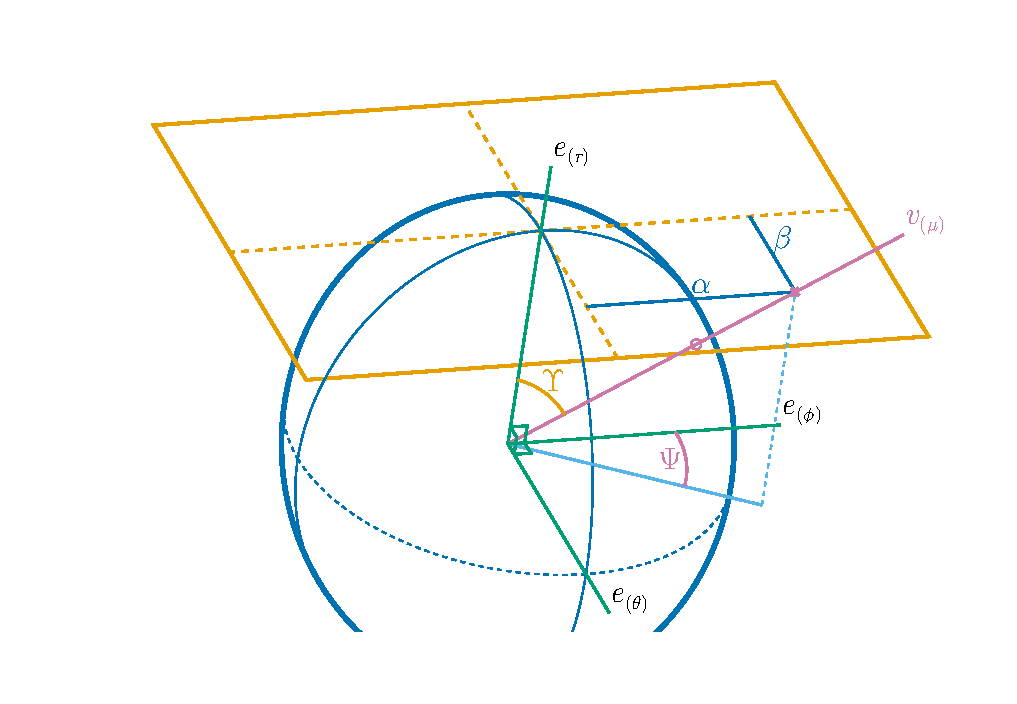
\includegraphics[width=0.99\linewidth]{figures/skycoords.pdf}
    \caption{
    Geometry of the local sky for an observer or emitter. The image plane (yellow) is
    perpendicular to the $e_{(r)}$ axis, which for an observer points towards
    the global origin and therefore the central singularity. The momenta
    $v_{(\phi)}$ and $v_{(\theta)}$ are used to calculate the impact parameters
    on the image plane, $\alpha$ and $\beta$ respectively. For emitters, the
    angles $(\Upsilon, \Psi)$ are used to parameterize points on the local sky,
    that may be decomposed onto the basis $e_{(i)}$ to find $v_{(\mu)}$.
    }
    \label{fig:observer-coordinates}
\end{figure}

We calculate the initial velocity $v^i$ differently depending on whether we are
considering an \emph{observer} or an \emph{emitter}.

For observers, we are interested in the sparse set of emitted photons which
reach an image plane representing the observer's field of view, and therefore
parameterize the velocity vector using \emph{impact parameters} on the image
plane. The parameters representing the local sky are shown in
Fig.~\ref{fig:observer-coordinates}, with the image plane drawn in yellow.
Following \cite{cunningham_optical_1973}, one may then define a set of
\emph{impact
parameters} from components of the local momenta $v_{(i)}$
\begin{align}
    \alpha &:=  x^r \frac{v_{(\phi)}}{v_{(r)}}, \\
    \beta &:= x^r \frac{v_{(\theta)}}{v_{(r)}},
\end{align}
using indices in parentheses to denote the vector components in the local
frame. The choice of subscript ($r, \theta, \phi$) is to anticipate identifying
coordinate directions in the local and global (metric) bases, and to suggest
some intuition for the meaning of directions in the local frame.

Exploiting the invariance of four-momenta (cf. Eq.
\eqref{eq:velocity_constraint}), we obtain a curve of solutions along $x^r$ for
the local momenta of geodesics intersecting the image plane at specific
$\alpha$ and
$\beta$
\begin{align}
    \frac{v_{(r)}}{v_{(t)}} &= -\left( \sqrt{1 + \left(\frac{\alpha}{x^r}\right)^2 + \left(\frac{\beta}{x^r}\right)^2} \right)^{-1} = \mathscr{R}, \\
    \frac{v_{(\theta)}}{v_{(t)}} &= \mathscr{R} \frac{\beta}{x^r}, \\
    \frac{v_{(\phi)}}{v_{(t)}} &= \mathscr{R} \frac{\alpha}{x^r}.
\end{align}
Note the choice of sign in the root of $v_{(r)} / v_{(t)}$, chosen so the
momentum points \emph{inwards} towards the black hole.

The case for emitters is subtly different, where we now consider polar and
azimuthal angles in the local sky, denoted $\Upsilon$ and $\Psi$ respectively (see
also Fig.~\ref{fig:observer-coordinates}). The momentum components are now
obtained by considering the tangent vector pointing in some initial direction;
that is, by projecting the initial velocity vector onto the local momentum
frame. This projection is compactly expressed as a decomposition onto a
Cartesian coordinate system
\begin{equation}
    \label{eq:local-angle-to-velocity}
    \frac{v_{(i)}}{v_{(t)}} = \frac{1}{v_{(t)}}
    \left[\pderiv{(x, y, z)}{(r, \theta, \phi)}\right]
    \left(
    \begin{matrix}
        \sin \Upsilon \cos \Psi \\
        \sin \Upsilon \sin \Psi \\
        \cos \Upsilon \\
    \end{matrix}
    \right),
\end{equation}
where the partial derivative matrix denotes the Cartesian to spherical
coordinate Jacobian. The component $v_{(t)}$ is the negative of the energy in
the local frame, and may be set to $-v_{(t)}=E=1$ without loss of generality.

The transformation between local and global frame depends on the choice of local
frame. The natural choice is the \emph{locally non-rotating frame}
\citep[LNRF;][]{bardeen_rotating_1972}. This frame follows strictly
circular world lines with $x^r = \text{const.}$ and $x^\phi = \omega t +
\text{const.}$, with angular velocity $\omega = -g_{t\phi} / g_{\phi\phi}$. The
coordinate transformation from the LNRF is
\begin{equation}
    \label{eq:local-to-global-velocity}
    v_\mu = \e^{(\nu)}_{\phantom{(\nu)}\mu}\  v_{(\nu)}
\end{equation}
where the local tetrad (basis vectors) $\e^{(\nu)}_{\phantom{(\nu)}\mu}$ are found
using the theorem of Gram-Schmidt (\citealp{schmidt_uber_1989}, Appendix
\ref{appendix:gram-schmidt}). The formalism may be extended for a local frame
in motion, where the frame velocity modifies the mapping by a local Lorenz
transformation, $\Lambda^{(\kappa)}_{\phantom{(\kappa)}(\nu)}$, as
\begin{equation}
    v_\mu = \e^{(\nu)}_{\phantom{(\nu)}\mu}\  \Lambda^{(\kappa)}_{\phantom{(a)}(\nu)} v_{(\kappa)}.
\end{equation}
This Lorenz transformation may be absorbed into the tetrad with careful
construction, mandating the velocity of the frame in the global coordinates as
$\utensor{\e}{(t)}{\mu}$ and orthogonalizing using the theorem of Gram-Schmidt.

These calculations may also be derived from the constants of motion that a
spacetime admits, $E$, $L$, and the Carter constant $Q$. The analytic
derivation of the LNRF and associated coordinate transformations is in
\cite{cunningham_optical_1973}. The authors derive the impact parameters under
the assumption that the observer is in asymptotically flat space, whereas our
calculations do not make this assumption. This allows us to use the impact
parameters anywhere in the spacetime, and approximate an asymptotically flat
space by positioning our observer at a large radial distance, say $r_\text{obs}
> 10^4 \rg$. This approximation incurs an error of order $\sim1/r_\text{obs}$
when compared to results using analytic derivations due to the energy and
angular momentum differing by a small amount in the global coordinates. This
must be taken into account when comparing GRRT codes to many decimal places.

\subsection{Special orbits and horizons}
\label{sec:special-orbits}

Of particular interest when studying accretion processes are the Keplerian
circular orbits, confined to the equatorial plane f$(x^\theta = \pi/2)$ in
axis-symmetric spacetimes. A subset of the Keplerian orbits are the circular
orbits, and are therefore relevant in analytical models of accretion discs
\citep{shakura_black_1973}. These circular orbits are stationary points of the
geodesic Hamiltonian, and constrained by $v^r = v^\theta = 0$.  These orbits are
often studied analytically, and have a general solution for metrics of the form
given by eq. \eqref{eq:stationary_axisymmetric_metric} (e.g.
\citealp{johannsen_regular_2013}, We provide a derivation with an extension
towards $a^\mu \neq 0$ in Appendix \ref{appendix:circular-orbits}).

Circular orbits are classified as either stable or unstable
\citep{wilkins_bound_1972,bardeen_rotating_1972}. There exists an innermost
stable circular orbit radius (ISCO, denoted $\risco$), below which orbits
are energetically hyperbolic: small perturbations will send test particles
escaping to infinity or spiralling into the central singularity. The stability of
an orbit depends on the sign of $\d E / \d x^r$, with $>0$ corresponding to
energetically stable configurations. The ISCO is the critical point at
which
\begin{equation}
    \label{eq:isco-definition}
    0 = \left. \frac{\d E}{\d x^r} \right\rvert_{x^r := \risco}.
\end{equation}
Stable circular orbits are only possible for radii $x^r \geq \risco$.  Within
the ISCO is the so-called \textit{plunging region} where $v^r \neq 0$.  Emission
from within the ISCO are generally disregarded in reflection and reverberation
models, though for specific disc models or inner boundary torques emission from
this region may be important (see e.g.
\citealp{reynolds_isco_1997,young_isco_1998, mummery_continuum_2024} for
emission contributions within the ISCO). For this reason, we make no concrete
assumptions about the plunging region, though will omit its contributions in
this paper.

The ISCO radius may be solved numerically when no analytic solution is known.
For stationary, axis-symmetric metrics, the energy of a given orbit is known from
\eqref{eq:energy-of-orbit}, with the derivative with respect to $x^r$
calculated using AD. We use the NonlinearSolve.jl package to perform the root
finding on the resulting expression \citep{Pal_NonlinearSolve_jl_2023}.

Stable orbits may also be determined purely from the numerical integration of
geodesics, by mandating a stability measure and optimizing the initial velocity
vector until some heuristic measure is a minimum. For example, let $\mathscr{M}$
measure the eccentricity of an orbit in the equatorial plane. For a given radius
$x^r$, the velocity corresponding to a circular orbit is $v^\mu = v^t \partial_t
+ v^\phi \partial_\phi $. With eq. \eqref{eq:velocity_constraint}, the circular
orbit velocity may be found through
\begin{equation}
    \underset{v^\phi}{\arg \min}\ \ \mathscr{M}(x^r, v^\phi),
\end{equation}
using a numerical optimizer. We use the Nelder-Mead simplex method as our
preferred optimization algorithm for exploring the $v^\phi$ parameter space
\citep{nelder_simplex_1965}. Due to only integrating finite windings of the
orbit, this approach may find both unstable and stable orbits. These are
distinguished by inspecting $E$ as a function of $x^r$, or similarly $E$ as a
function of $L_z$ \citep{hackmann_charged_2013}, see Figure \ref{fig:e-lz-cusp}.
The $\risco$ is found by solving eq. \eqref{eq:isco-definition} numerically, or
by finding $x^r$ corresponding to the \emph{cusp} of the curve of  $E$ against
$L_z$.

\begin{figure}
    \centering
    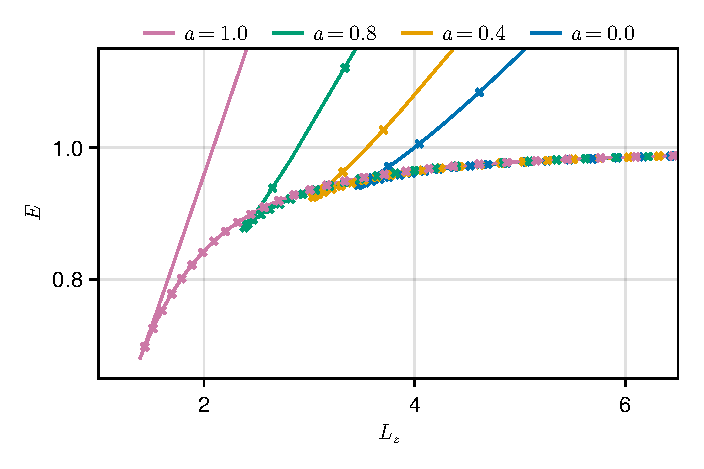
\includegraphics[width=0.95\linewidth]{figures/circular-orbits.E-Lz.pdf}
    \caption{Energy $E$ and angular momentum $L_z$ for (stable) circular orbits
        in the Kerr spacetime for different black hole spins. The point
        corresponding to the sharp cusp is the ISCO. The crosses show the $E$
        and $L_z$ values calculated by optimizing the stability condition (see
        text for details). For the maximally spinning spacetime, the optimizer
        is unable to find solutions within the ISCO, as the ISCO exactly
        coincides with the coordinate singularity corresponding to the event
        horizon.}
    \label{fig:e-lz-cusp}
\end{figure}

The velocities of orbits in the plunging region are numerically calculated by
``dropping'' a test particle from $\risco -  \delta x^r$, and tracing for a
large interval of proper time, until the fate of the geodesic is realized. The
components of $v^\mu$ are then interpolated over $x^r$ to approximate analytic
solutions. Figure \ref{fig:circular-orbit-error} illustrates the accuracy of our
numerical method for determining such plunging orbits.

This heuristic optimization technique is also used for other objective
functions, such as for solving for the initial conditions of  geodesics that
intersect a chosen point in the spacetime ($\mathscr{M}$ measures closest
approach), or that exhibit some specific desired features (e.g. $\mathscr{M}$
measures periodicity).

We implement a numerical method for determining the event horizon radius using a
similar approach. Under axis-symmetry, the event horizon is the set of $(r,
\theta)$ coordinates that satisfy
\begin{equation}
    \label{eq:event_horizon}
    0 = \left. \frac{1}{g_{rr}} \right\rvert_{x^r =: r_s}.
\end{equation}
For the cases where no analytic solution is known, we fallback to solving for
the event horizon using the root finding method as for the ISCO.

\subsection{Charts and horizons}

The chart defines the boundary of the integration used by the integrator to
terminate the computation when the fate of a given geodesic is known. In
practical terms, the chart is a set of callbacks in the integrator that mark the
union of a set of boundaries, intersection with which classifies the outcome of
an integration (e.g. geodesic is within the horizon, escaped to infinity,
intersected with disc, and so on). In the majority of cases, the inner and outer
boundary of the integration chart are the event horizon $r_s$ and some
\emph{effective infinity} $r_\infty$ respectively. In the latter case, the
geodesic is assumed to escape the potential of the singularity without further
deviation it their trajectory.

The geometry of an accretion disc or object is also expressed as a boundary of
the chart. By terminating the integration when the geodesic crosses such a
boundary, we consider the geodesic to have intersected the surface of the
accretion disc, and mark it accordingly. The marks are later used to group
geodesic solutions together when calculating physical quantities and
observables.

Close to the inner radius the adaptive time step of certain ODE integrator
algorithms tends to shrink dramatically due to near-singular derivatives,
causing the integration to slow to almost a standstill, and therefore becomes
very computationally expensive. We avoid this by scaling the inner horizon
with the choice of a constant $\mathcal{K} > 0$, such that $\tilde{r}_s = (1 +
\mathcal{K}) r_s$, terminating the integration when $x^r \leq
\tilde{r}_s$. This constant may be adjusted depending on the interest
in probing that region of the spacetime. We choose $\mathcal{K} =
10^{-2}$ by default to improve performance without no impact on the majority of
simulations.

The points of intersection with a Chart are found using either the interpolating
root-solver in \texttt{ContinuousCallback} or a per-point test with
\texttt{DiscreteCallback}, both made available from DifferentialEquations.jl
\citep{rackauckas_differential_2017}.

\subsection{Computing observables}
\label{sec:computing-observables}

In \Gradus, an \textit{observable} is any physical quantity calculated from a
simulation. Computing an observable requires some or all points $p = (x^\nu,
v^\nu)$ along a geodesic, though often only the start and end points are
required. In such circumstances, some computational concessions may be made to
save memory allocations. Observables are abstracted in the implementation, and
depending on the observable being calculated, different parts of the geodesic
are held in memory during integration.

An observable that requires multiple points along the geodesic can be calculated
either coincidentally with the geodesic equation\footnote{The ODE system is then
modified with an additional differential equation representing the observable.},
or subsequently re-traced along the ray. Such quantities include polarization /
parallel transport angle or radiative transfer intensities. Calculating the
quantities simultaneously has the benefit that the error tolerance in the
integrator is sensitive to changes in the observable. The benefit of re-tracing
for a given set of metric parameters and observer inclination is that the
geodesics trajectories are unchanged, allowing the observable to be more
efficiently recalculated with new parameters.

The redshift $g$ along a geodesic is an observable that only requires the start
and end points of a geodesic. The redshift includes both the Doppler shift and
gravitational redshift, and is compactly written as the ratio of energies
between the start and end point,
\begin{equation}
\label{eq:redshift}
g := \frac{E_\text{end}}{E_\text{start}} = \frac{\left. v_\mu u^\mu
\right\rvert_\text{end}}{\left. v_\mu u^\mu \right\rvert_{\text{start}}},
\end{equation}
where $v_\mu$ are the geodesic momenta, and $u^\mu$ the velocity of the emitting
(start) and observing (end) media respectively.



\subsection{Disc illumination and emissivity profiles}
\label{sec:emissivity-profiles}

The \emph{illumination profile} is the local flux of radiation on the disc as a function of radius, $\varepsilon(r)$, for an axis-symmetric system. This is often referred to as the \emph{emissivity profile} as the line strength in the back-scattered spectrum is often proportional to the illuminating flux.
The illumination profile is related to the ionization parameter, $\xi(r)$, of the accretion disc \citep{laor_line_1991,ross_reflection_1993, wilkins_understanding_2012}
given by
\begin{equation}
    \xi = \frac{4 \pi F_i}{n_\text{H}}
\end{equation}
where $F_i$ is the total illuminating X-ray flux in some band, often $0.01 - 100 \text{ keV}$, and $n_\text{H}$ is the co-moving hydrogen density \citep{ross_effects_1993}.
For our purposes, we will drop factors considered to be constant, and use
$\varepsilon \propto F_i$ directly.

The source of $F_i$ is a luminous corona located close to the central
singularity \citep{svensson_corona_1994}, often assumed to be a point source on the spin axis of
the black hole that emits isotropically, resulting in an $F_i$ that is
axisymmetric. This model is known as the ``lamppost'' coronal model
\citep{fukumura_accretion_2007}. Axisymmetric extended coronae are also
considered, and in general the morphology of the corona has a significant effect
of the emissivity profile \citep{wilkins_towards_2016, gonzalez_probing_2017}.
For axisymmetric corona with isotropic emissions, the incident flux (and
therefore the emissivity profile), is a function of only the cylindrical
coordinate on the disc $\rho = r \sin(\theta)$. The flux in an annulus is the
number density of photons in the annulus along with an intensity function $I$
representing the emission spectrum of the corona.  Therefore, up to a constant
of proportionality, the emissivity function is
\begin{equation}
    \varepsilon (\rho, \d \rho) = \frac{\mathcal{N}(\rho, \d \rho)}{\gamma
    \tilde{A}(\rho, \d \rho)} I(g),
\end{equation}
where $\mathcal{N}$ is the geodesic count in an annulus $\rho + \d \rho$, $I$ is
the intensity of the illuminating flux as a function of redshift $g$,
$\tilde{A}$ is the curvature corrected (proper) area of the annulus, and
$\gamma$ is the Lorentz factor that accounts for area contraction of the annulus
due to the velocity of the disc.

The relativistic corrections are as follows: for an infinitesimal area $\d A = \d
\rho\d\phi$, the \textit{proper area} is calculated directly from the metric,
and so
\begin{equation}
    \d\tilde{A} = \sqrt{g_{rr} g_{\phi\phi}}\, \d \rho\, \d \phi,
\end{equation}
is the area as measured by a stationary observer in the disc. The relativistic
Lorentz factor is calculated as
\begin{equation}
    \gamma = \frac{1}{\sqrt{1 - \left(v^{(i)}\right)^2}},
\end{equation}
where $v^{(i)}$ are the spatial components of the angular velocity in the LNRF.
These components are determined for a given basis
\begin{equation}
    v^{(i)} = \frac{\utensor{\e}{(i)}{\mu}\, v^\mu}{\utensor{\e}{(t)}{\sigma}\, v^\sigma},
\end{equation}
where the special case of circular orbits in the equatorial plane only has
$v^{(\phi)}$ non-zero.

The emission spectrum for the illuminating corona is usually assumed to be a
powerlaw $I(g) = g^{-\Gamma}$ with photon index $\Gamma$ For most applications
$\Gamma = 2$ or $3$ is chosen \citep{mushotzky_agn_pl_1982,remillard_binaries_2006}. Our models make no rigid assumptions
about the coronal spectrum, and any arbitrary spectrum as a function of $g$ may
be specified.

When the emission from the corona is assumed to be locally isotropic in the rest
frame of the corona, geodesics from the source are traced by sampling
$(\Upsilon, \Phi)$ evenly on a sphere. The angles are transformed via equations
\eqref{eq:local-angle-to-velocity} and \eqref{eq:local-to-global-velocity} to
find the initial velocity of the geodesic. Those geodesics that intersect with
the disc are then used to calculate the emissivity. When the emission in
non-isotropic, the sampled distributions of $(\Upsilon, \Phi)$ are appropriately
weighted. The geodesics followed until they are terminated by one of the domain
boundaries, and those that intersect with the accretion disc are used to
determine the photon number density.

For axis-symmetric point-source corona, the irradiating flux may alternatively
be determined by exploiting symmetries as in \cite{dauser_irradiation_2013}. A
set of photons with different polar angle $\Upsilon$, spaced evenly with some
$\Delta \Upsilon$, are traced and used to determine the radial boundaries of the
annuli on the disc, each with some width $\Delta r$ which acts as a proxy for
reciprocal photon number density, i.e. $\Delta r \propto 1 / \mathcal{N}$. In
three spatial dimensions, the polar coordinate must be distributed as $\sin
\Upsilon$ for isotropic emission, and therefore $\varepsilon$ is weighted
similarly,\footnote{Instead of equally spaced $\Upsilon$, one may instead sample
$\Upsilon \sim \cos (1 - 2 \mathcal{U})$, where $\mathcal{U}$ is a uniform
distribution $\mathcal{U}(0,1)$. In this case, there is no $\sin \Upsilon$
weight in $\varepsilon$. This result may be shown using the inverse-CDF or
Smirnov transform method.}
\begin{equation}
    \varepsilon(r, \Delta r) = \frac{\sin \Upsilon}{\gamma \tilde{A}(r, \Delta r)} I(g).
\end{equation}
An illustration of the two methods is shown in Figure \ref{fig:coronal-tracing}.
It should be noted that the latter method converges faster than the
former (Monte-Carlo) sampling approach, and captures the behaviour at small $r$
close to the ISCO faithfully -- behaviour that would otherwise require an
inordinate number of samples. However, since this method is specialized for
point sources, extended coronae require an approximate rebinning algorithm to
reconstruct the emissivity profile taking into account the overlap between the
annuli determined from different source points.

\begin{figure}
    \centering
    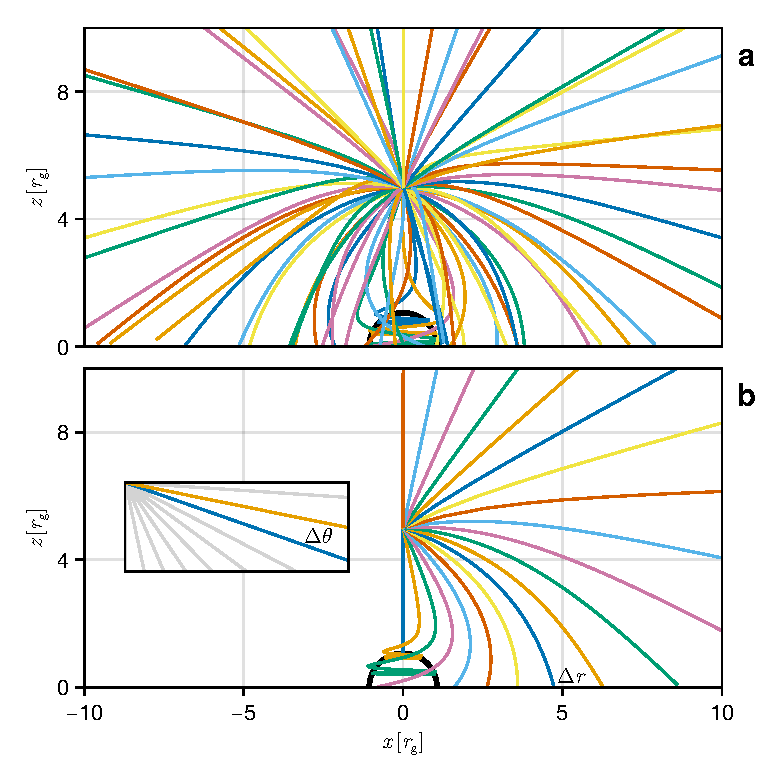
\includegraphics[width=0.95\linewidth]{figures/emissivity.coronal-traces.pdf}
    \caption{An illustration of the methods described in the text for
        calculating the emissivity of a lamppost corona: the colourful lines are
        the null-geodesics of a lamppost model illuminating the accretion disc
        around in a maximally spinning Kerr spacetime ($a = 0.998$). Panel a) is
        the Monte-Carlo approach, where the initial velocity vector of the
        photon is sampled isotropically on the local sky of the emitter. The
        number density on the disc in a given annulus is then used as a proxy
        for the flux density. Panel b) shows how the symmetry of the lamppost can
        be exploited, by considering only a slice of the emission around the
        spin axis. The initial velocity vectors now differ by a constant $\Delta
    \theta$, which allows the spacing on the disc $\Delta r$ to be used as a
proxy for flux density.}
    \label{fig:coronal-tracing}
\end{figure}

When axis-symmetry does not apply, we have developed a method for calculating
the emissivity field as a function of $(r, \phi)$ on the disc by treating the
points of intersection as the generators of a Delauney tesselation. The
(relativistically corrected) Voronoi area may be used as a proxy for the photon
number density $\mathcal{N} /\tilde{A}$  in the limit of high sample count (see
Appendix \ref{appendix:voronoi}).

\subsection{Transfer functions}
\label{sec:transfer-functions}

\begin{figure*}
    \centering
    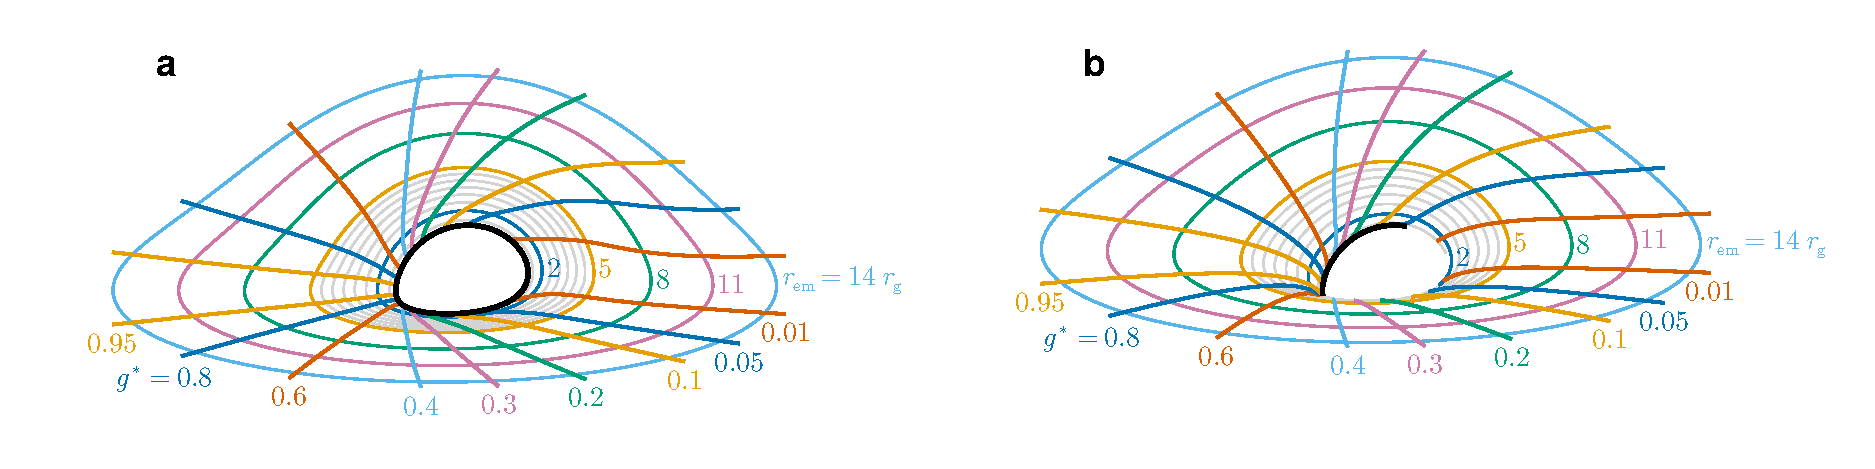
\includegraphics[width=0.95\linewidth]{figures/transfer-function.parameterization.pdf}
    \caption{Concentric rings of radius $r_\text{em}$ and contours of constant
    dimensionless redshift $g^\ast$ on disc in the equatorial plane, projected
on the image plane of a distant observer at $\theta_\text{obs} = 75^\circ$. The
central singularity is described by the Kerr metric with $a = 0.998$. The
innermost thick black line is the projection of the ISCO. Note the contours of
$g^\ast$ are double valued for any given $r_\text{em}$. Panel a) geometrically
thin disc. Panel b) \citet{shakura_black_1973} Disc (SSD) with $\dot{M} / \dot{M}_\text{Edd} = 0.3$, with
obscuration of some of the inner radii. The edge of the ISCO is here only
partially visible.}
    \label{fig:transfer-parameterisation}
\end{figure*}

To motivate the use of \emph{transfer functions}, consider the calculation of an
observed spectrum of flux reflected by the accretion disc. The infinitesimal
flux element, $\d F(E)$, is related to the specific intensity in the solid angle element
\begin{equation}
\label{eq:infinitesimal-flux}
\d F(E) = I(E)\, \d \Omega,
\end{equation}
for observed energy $E$, specific intensity $I$ and solid angle $\d \Omega$.
\cite{cunningham_effects_1975} gives an intuitive relation between the observed
and emitted intensities as derived using the \emph{reciprocity theorem} \citep[or
equivalently \emph{Liouville's theorem};][]{lindquist_louville_1966} with
\begin{equation}
\label{eq:liouville-theorem}
I_\text{obs}\left( E_\text{obs}\right) = g^3 I_\text{em}\left(E_\text{em}\right).
\end{equation}
Integrating over $\d \Omega$ to obtain the observed flux $F(E_\text{obs})$ is
equivalent up to a constant to integrating over the image plane $\d \alpha \d
\beta$,
\begin{equation}
\label{eq:integrate-impact-params}
F(E_\text{obs}) \propto \int I_\text{obs}(E_\text{obs}) \d \alpha \d \beta,
\end{equation}
which in practical terms is binning the geodesic in each pixel over bins of
$\Delta E$.  Formulating the flux calculation in this way is computationally
simple but expensive, as the flux is computed on a pixel-by-pixel
(geodesic-by-geodesic) basis. The emitted intensity $I_\text{em}$ depends on the
disc emissivity, requiring both coordinate and redshift values for each geodesic
to be stored to compute the flux. These quantities are dependant on the metric,
disc, and observer parameters, and this dependence limits the reuse of
calculations between simulations, undesirable for creating spectral models.

To elide such problems, the relativistic effects in the flux calculation are
often encoded in so-called \emph{transfer functions}
\citep{brenneman_constraining_2006}. The most ubiquitous formulation of these
transfer functions was first introduced in \cite{cunningham_effects_1975}.
There, they are defined
\begin{equation}
    \label{eq:cunn-transfer-function}
    f:=\frac{g}{\pi r_\text{em}} \sqrt{g^\ast(1 - g^\ast)} \jacobian{(\alpha, \beta)}{(r_\text{em}, g^\ast)},
\end{equation}
where $r_\text{em}$ is the emission radius on the disc, and
\begin{equation}
    g^\ast := \frac{g - g_\text{min}}{g_\text{max} - g_\text{min}} \in [0, 1],
\end{equation}
is a rescaled dimensionless redshift parameter. The extremal values of $g$ are
calculated over a given emission radius on the disc, $r_\text{em}$.

The parameterization of $g^\ast$ is double-valued everywhere except at $g^\ast =
0$ and $1$, with the two branches of $g^\ast$ being attributed to the sections of the
disc closest and furthest from the observer. This naturally leads to the
interpretation of the Cunningham transfer functions as recasting the projection
of the accretion disc on the image plane from $(\alpha, \beta)$ to
$(r_\text{em}, g^\ast)$, see Figure \ref{fig:transfer-parameterisation}.  The
additional elliptical envelope in $g$ suppresses the singular values of the
Jacobian as $g^\ast$ becomes $0$ or $1$, resulting in numerically better behaved
functions at extremal $g^\ast$.

As a note, the name \emph{transfer functions} is a more general term and used
elsewhere, for example in reverberation simulations discussed later. To avoid
ambiguity, we henceforth refer to functions of the kind defined in equation
\eqref{eq:cunn-transfer-function} as \emph{relativistic} or \emph{Cunningham
transfer functions}. Furthermore, the Cunningham transfer functions are referred
to as having ``upper'' and ``lower'' branches between extremal $g^\ast$, as
shown in Figure \ref{fig:transfer-functions}, stemming from the double-valued
nature of $g^\ast$. When the emission from the disc is not isotropic, the
distinction between these branches becomes important. Cunningham transfer
functions also make a number of assumptions about the system under
consideration, principally that only one side of the disc contributes to the
flux (no false images), and, as we shall see, do not generalize to thick discs
easily. Nevertheless, when these assumptions apply, the Cunningham transfer
functions provide a number of significant benefits over the naive binning
approaches.

Integrating $f$ over $(\d r_\text{em}, \d g^\ast)$ is then equivalent to
integrating over the image plane for only those photons that are coming from the
disc. The Cunningham transfer functions are therefore a sparse way of encoding
the full image plane in a manner that allows for efficient integration.

\subsubsection{Calculating Cunningham transfer functions}

Before integrating the Cunningham transfer functions, we must first calculate
them. Our method for calculating $f$ is a variation of the algorithms of other
authors (\citealp{speith_photon_1995,bambi_testing_2017}, improved in
\citealp{abdikamalov_public_2019}), and uses AD to compute the Jacobian term.

The procedure is as follows: first, we find the impact parameters that map to a
ring of radius $r_\text{em}$ on the accretion disc. In the case of simple
axis-symmetric discs, the projection of a ring will be the boundary of a
star-convex set on the image plane, and therefore a polar curve
$\mathcal{R}(\vartheta)$, with $\alpha = \mathcal{R}(\vartheta) \cos(\vartheta)$
and $\beta = \mathcal{R}(\vartheta) \sin(\vartheta)$. For a given $\vartheta$,
the offset on the image plane $\mathcal{R}$ is found by root-finding the
difference between $r_\text{em}$ and the projected endpoint of the geodesic on
the disc $r = x^r (\mathcal{R}) \sin x^\theta(\mathcal{R})$, using the same
alternating root-finder as in Section \ref{sec:special-orbits}.

Then we must determine the extrema of $g$ over the $r_\text{em}$ ring. The
extremal $g$ are found by using the Golden-Section bracketing method of
\cite{Optim.jl-2018} to extremize $g(\vartheta)$, solving a new geodesic
at each step. We make the assumption that extremal $g$ approximately coincide
with extremal $\beta = 0$, and therefore shift the domain to $\vartheta \in [
-\pi/2, 3\pi/4)$ to ensure the maxima and minima are away from the edges of the
domain to help the optimizer.

The importance of accurately calculating $g_\text{min}$ and $g_\text{max}$ is
difficult to overstate: small errors here will dramatically alter the shape of
the transfer functions close to $g^\ast \rightarrow 0$ and $g^\ast \rightarrow
1$, and have a high likelihood of sending $f$ to positive or negative infinity.
Even when the extrema are determined to high accuracy, in practice, it is useful
to employ a small truncation of $\delta g^\ast = h \sim 10^{-6}$ either side
of the domain when doing anything practical. This is discussed in the next
section in further detail in the context of integrating $f$.

Finally, the Jacobian is calculated by retracing all previously traced $(\alpha,
\beta)$ that map to $r_\text{em}$ with AD. Other authors will here use
\begin{equation}
    \left\lvert
    \pderiv{(\alpha, \beta)}{(r_\text{em}, g^\ast)}
    \right\rvert
    =
    \left\lvert
    \pderiv{r_\text{em}}{\alpha}\pderiv{g^\ast}{\beta}
    -
    \pderiv{r_\text{em}}{\beta}\pderiv{g^\ast}{\alpha}
    \right\rvert^{-1},
\end{equation}
and determine the derivatives with a finite difference stenciling approach, or
even use a fixed $\delta \alpha$ and $\delta \beta$. Unless the algorithm can
adapt extremely well, this approach may introduce singular values or risk large
numerical error at extremal $g$. AD avoids some of these problems, and has the
additional benefit that it only requires the evaluation of a single geodesic to
compute, and is thus substantially faster.

The total number of geodesics traced for each Cunningham transfer function
depends on the number of steps needed to solve impact parameters for a given
$r_\text{em}$, and on the number of steps needed to extremize $g^\ast$ to within
some tolerance. In our code, we set an upper-limit on the number of steps so
that memory can be contiguously allocated, and the cost of curtailing some
calculations. Our default configurations use an upper limit of $N = 114$ points
along $r_\text{em}$, $80$ of which are approximately linearly sampled in
$\vartheta$, and $34 = 2 \times 17$ used to determine $g_\text{min}$ and
$g_\text{max}$. These limits were chosen to balance speed and accuracy of
calculation. The resulting sampling pattern is sensitive to various extrema in
$g$, and determines the shape of $f$ well, as shown in Figure
\ref{fig:transfer-sampling-pattern}.

\begin{figure}
    \centering
    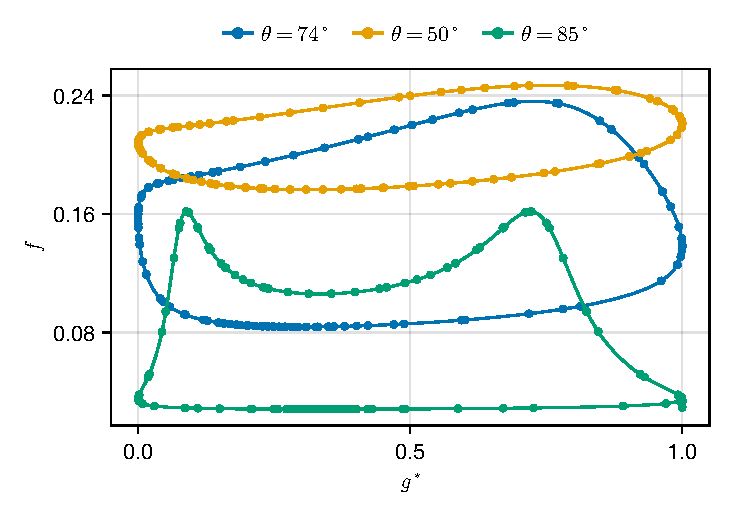
\includegraphics[width=0.95\linewidth]{figures/transfer-functions.sampling.pdf}
    \caption{Transfer functions of the Kerr spacetime ($a = 0.998$) for various
        observer inclinations, showing the sample pattern of $g^\ast$ that our
        algorithm (described in the text) produces. The higher
        density of points around extremal $g^\ast$ is due to the optimizer we
        employ to determine the extremal points. Note that for the high
        inclination case ($\theta = 85^\circ$) there is slight numerical noise
        very close to $g^\ast = 1$. This noise is in the region excluded by the
        integration scheme, and therefore contributes negligible error in
        calculations involving transfer functions. There is also a high density
        of points on the lower branch of the transfer function, which is an
        artefact of the projection of the disc onto the observer's plane.
    }
    \label{fig:transfer-sampling-pattern}
\end{figure}

\subsubsection{Partially obscured Cunningham transfer functions}
\label{sec:partially-obscured-functions}

For thick accretion discs, it is possible that the disc obscures itself, and
that certain $r_\text{em}$ may therefore be only partially visible or entirely
obscured to an observer at inclination $\theta_\text{obs}$ (see Figure
\ref{fig:transfer-parameterisation}b). When this is the case, the method of
calculating Cunningham transfer functions is modified through the use of
\emph{datum planes}.

We define a \emph{datum plane} to be an infinite plane at some scale height
$z_\text{em} = r_\text{em} \cos \theta$, and used as the manifold over which the
optimizer solves the projection of the ring at $r_\text{em}$. The datum plane
is in essence a cut-off for integration such that all geodesics terminate with
the same $z$, see Figure \ref{fig:datum-plane-tracing}.

As before, we determine the extremal redshift over the ring $r_\text{em}$,
including those geodesics from obscured regions of the disc. As the redshift
depends only on the start and end point of the geodesic, it is therefore simpler
to combine this with the radius-solving step and calculate the redshift over the
datum plane. This is not so for the Jacobian term, which depends on the cross
section traced by a bundle of geodesics for which the geometry of the disc is
important. The Jacobian is calulated by tracing against the thick disc and is
combined with a check to see if a patch of the disc is obscured. This
obscuration check is used to mask the transfer functions, as in Figure
\ref{fig:transfer-functions}. This method is in effect analogous to the
``imaginary photons'' of \cite{abdikamalov_testing_2020}, formalized for
optimizing $r_\text{em}$ and AD.

\begin{figure}
    \centering
    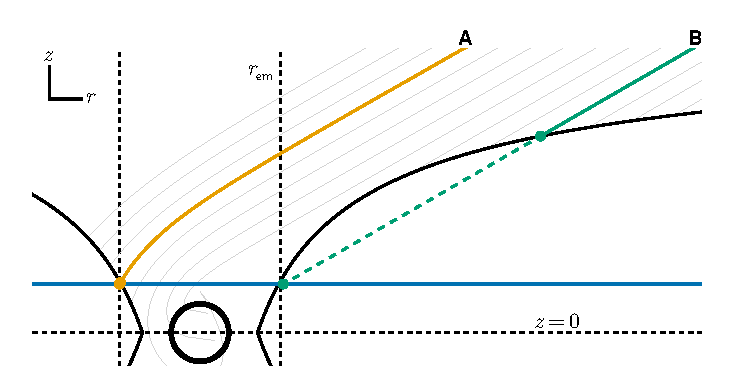
\includegraphics[width=0.95\linewidth]{figures/datum-plane.pdf}
    \caption{Cross-sectional slice of geodesics traced from a distant observer
        against a datum plane (horizontal blue line) through a thick disc
        (curved black line). The observer ``sees'' the solid geodesics
        intersecting the disc, whereas for the purposes of calculating the
        Cunningham transfer functions, we continue integrating along the dashed
        line until intersecting the datum plane. For geodesic A the observer
        can see the emission radius $r_\text{em}$, whereas for B the radius is
        obscured.
}
    \label{fig:datum-plane-tracing}
\end{figure}


\begin{figure*}
    \centering
    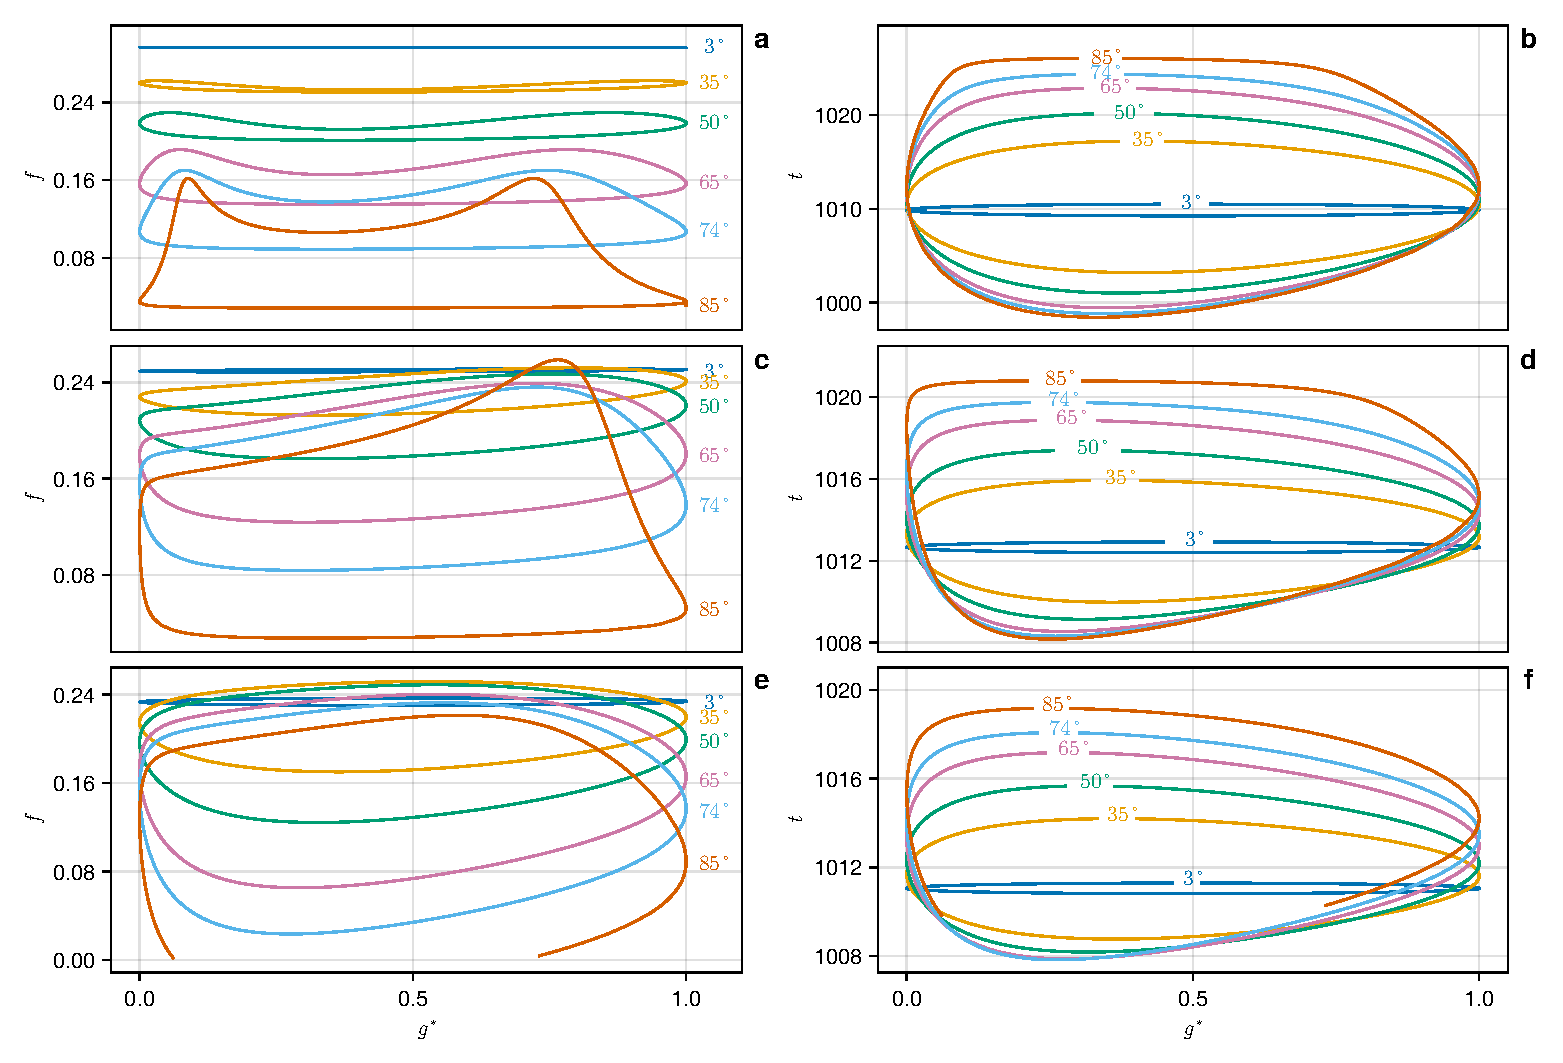
\includegraphics[width=0.99\linewidth]{figures/transfer-functions.plots.pdf}
    \caption{Transfer functions $f$ and timing $t$ for fixed $r_\text{em}$ for different observer inclinations $\theta_\text{obs}$ and $r_\text{obs} = 10^3 \rg$. Panels a) and b) Schwarzschild spacetime with equatorial thin disc and $r_\text{em} = 11\, \rg$. Panels c) and d) Maximally spinning Kerr spacetime $a=0.998$ with equatorial thin disc and $r_\text{em} = 4 \, \rg$ (see also \citealp{bambi_testing_2017}, their Figure 1). Panel e) and f) Maximally spinning Kerr spacetime $a=0.998$, with SSD $\dot{M} / \dot{M}_\text{Edd} = 0.3$ and $r_\text{em} = 4\, \rg$, showing obscuration at steep inclination.}
    \label{fig:transfer-functions}
\end{figure*}

\subsection{Integrating transfer functions}
\label{sec:transfer-function-integration}

Using the Cunningham transfer functions as a Jacobian allows us to rewrite the
integration \eqref{eq:integrate-impact-params} as
\begin{equation}
    F(E_\text{obs}) = \int \frac{\pi r_\text{em} f(r_\text{em}, g^\ast)}{g \sqrt{g^\ast (1 - g^\ast)}}
    I_\text{obs}(E_\text{obs}) \ \d r_\text{em} \d g^\ast,
\end{equation}
where we can use Liouville's theorem \eqref{eq:liouville-theorem} to express the
observed intensity in terms of the emitted intensity, and write $E_\text{obs} =
E_\text{line}g$ . The integrand is then only a function of $r_\text{em}$ and
$g^\ast$. We here see a new meaning for the Cunningham transfer functions,
namely as the Green's function of an annulus $r_\text{em}$ in response to some
delta function of $I_\text{em}$. This interpretation is used to guide
integration schemes for the transfer functions \citep{dauser_broad_2010}.

The Cunningham transfer functions are split into the aforementioned
upper and lower branches at extremal $g^\ast$, and each branch is integrated
separately, with the total summed in the final result. We extend the transfer
function integration to include the geodesic coordinate time, resulting in the
integral
\begin{align}
    \label{eq:transfer-integration}
    F(E, t) &=
    \pi
    \int_0^\infty \d t^\prime \delta(t - t^\prime)
    \int_{r_\text{in}}^{r_\text{out}} \d r_\text{em}\,r_\text{em} \nonumber \\
    &\ \int_0^1 \d g^\ast\, \delta(E - gE_\text{line})\, g^2 I_\text{em}\left(\frac{E}{g}, t^\prime\right) \frac{f(r_\text{em}, g^\ast)}{\sqrt{g^\ast (1 - g^\ast)}},
\end{align}
denoting $g = g( r_\text{em}, g^\ast, t')$ implicitly. We use the Dirac delta
functions to select the $E$ and $t$ bins of the observed flux respectively,
however we note that at no point can we continuously evaluate the integrand, and
this notation serves only to express what we are trying to do. In practical
terms, we have a discrete set of Cunningham transfer functions over which can
can smoothly interpolate. The method for numerically integrating the
time-dependent transfer functions is as follows: the limits of the integral are
chosen $(r_\text{in}, r_\text{out})$, as are the limits of the output space
similarly $(E_\text{min}, E_\text{max})$, $(t_\text{min}, t_\text{max})$. Any
evaluation of \eqref{eq:transfer-integration} that is outside of the energy and
time limits is discarded. The integration over $\d r_\text{em}$ is performed
using a trapezoidal scheme, as it is found to be sufficient in both accuracy and
performance. For the integration over $\d g^\ast$ we must be more careful.

The $\d g^\ast$ quadrature scheme evaluates $F(E)$ for each branch over a small
output bin in $g$, such that $t$ is determined by evaluating $t(g^\ast)$ at the
limits of the bin, also for each branch. These approximations mandate that the
integration is performed over a fine $g$ grid. In full:
\begin{enumerate}
    \item Interpolate the values of the transfer function, $f$, $t$, and
        $g_\text{min}$, and $g_\text{max}$, for the current radius $r_i$.
    \item Calculate the trapezoidal integration weight for the radial coordinate
        $\omega_i = \Delta r_i r_i$. Any other quantities that only depend on
        $r_\text{em}$ may similarly be factored into this weight, e.g. if
        $I_\text{em} = I_\text{em}(r_\text{em})$.
    \item For each bin in the fine $g$ grid, integrate $f$ over this bin. Record
        $t_\text{min} = t(g_\text{min})$ and $t_\text{max} = t(g_\text{max})$.
        Note that depending on the interpolation scheme, if $f$ is a function of
        $g$ instead of $g^\ast$, a $g / (g_\text{max} - g_\text{min})$
        change-of-variable factor must be included in the integrand.
    \item Add $\omega_i F_i(E, t)$ to the bin corresponding to $E =
        gE_\text{line}$, and $t(g^\ast)$ for each branch. If either $\Delta E$
        or $\Delta t$ straddles an output bin, the flux must be weighted
        appropriately and divided into those bins.
\end{enumerate}

The integrand for each branch remains in practice singular at $g^\ast
\rightarrow (0, 1)$, and therefore the integration is performed over $g^\ast \in
[h, 1 - h]$. Outside of this domain, the limits of the integrand can be taken to
approximate the edges of the bin, as in \cite{dauser_broad_2010},
\begin{equation} F_\text{edge}(E,t) \propto 2\left( \sqrt{E_\text{max}} -
\sqrt{E_\text{min}} \right).  \end{equation} The constant of proportionality is
determined from evaluating the integrand at $h$ or $1 - h$ respectively.

We use $h = 2 \times 10^{-6}$, and evaluate the integral over $\d g^\ast$ using
a 7$^\text{th}$ order Gauss-Kronrod quadrature scheme, which avoids evaluating
the integral directly at $h$ and $1 - h$. Finer grids for $r_\text{em}$
and $g^\ast$ are constructed to help with numerical accuracy and stability, with
the finer bins subsequently rebinned into the desired output grid\footnote{The
    grid in $r$ should be regularly spaced, e.g. $\sim 1 / r$, reflecting the
    fact that the majority of the variation in $f$ occurs at small $r$. For
$g^\ast$, the variation is approximately uniform over the domain, and so we use
a uniform grid of $N = 30$ points over $g^\ast$. This also make saving the
transfer functions in a tabular format simple.  }.

By formulating the Cunningham transfer function integration with the time
component, we can use the same transfer function table to compute both
line-profiles and timing properties (e.g., X-ray reverberation lags) efficiently, with arbitrary intensity
functions $I_\text{em}$. We note that extensions to $I_\text{em}$ that require,
for example, the photon emission angle on the disc $\mu = \cos(\theta)$ \citep{matt_reflection_1993}, are
simple to include.

% These transfer function integration methods may be checked for consistency
% against slower but simpler direct binning of the image plane via Eq.
% \eqref{eq:infinitesimal-flux} and Eq. \eqref{eq:liouville-theorem}.

\subsection{Covariant radiative transfer}

The intensity of a given geodesic is an observable that can be either calculated coincident with the geodesic trajectory, or retraced once the trajectory is determined.

The covariant formulation of the radiative transfer equation calculates the emissions and extinction in aframe co-moving with the geodesic \citep{fuerst_radiation_2004,younsi_general_2012}. The generalized form of the differential equation with respect to the affine parameter $\lambda$ is
\begin{equation}
    \label{eq:covariant-radiative-transfer}
    \frac{\d \mathcal{I}}{\d \lambda} = \left. \frac{\d s}{\d \lambda} \right\rvert_\lambda \left( -\alpha_\nu \mathcal{I} + \frac{j_\nu}{\nu^3} \right),
\end{equation}
where $\mathcal{I}$ is the invariant intensity, $s$ is the proper length traversed by the geodesic, and $\alpha_\nu$ and $j_\nu$ are the frequency $\nu$ dependent absorption and emissivity coefficients respectively, as measured in the local frame. The frequency $\nu$ is related to the observed frequency via the redshift
\begin{equation}
    g = \frac{\nu_\text{obs}}{\nu},
\end{equation}
In general, both coefficients $\alpha_nu$ and $j_\nu$ are also functions of the position $x^\mu$.

The $\d s / \d \lambda$ derivative term is calculated by projecting the geodesic momentum $v_\mu$ onto the velocity $u^\mu$ of the medium, using the projection tensor
\begin{equation}
    \mathrm{P}^{\mu\nu} := g^{\mu\nu} + u^\mu u^\nu.
\end{equation}
The path length derivative is
\begin{align}
    \left. \frac{\d s}{\d \lambda} \right\rvert_\lambda
    &= - \left. \left\lVert \mathrm{P}^{\mu\nu} v_\mu\right\rVert\, \right\rvert_\lambda,\\
    &= - \left. \sqrt{v_\mu v^\mu + \left(v_\mu u^\mu\right)^2 \left(2 + u^\mu u_\mu\right)} \, \right\rvert_\lambda,
\end{align}
such that for the particular case of null geodesics through a time-like medium
\begin{equation}
    \left. \frac{\d s}{\d \lambda} \right\rvert_\lambda = - \left. v_\mu u^\mu \right\rvert_\lambda.
\end{equation}

The covariant intensity $\mathcal{I}$ is related to the observed intensity $I_\nu = \mathcal{I} \nu^3$, derived using Liouville's theorem \citep{todo}. The intensity is therefore calculated by selecting $\nu_\text{obs} = E$ at the observer, and integrating \eqref{eq:covariant-radiative-transfer} along a given geodesic.


%%% DESCRIPTION OF THE CODE %%%%%%%%%%%%%%%%%%%%%%
\section{Description of the code}
\label{sec:description-of-code}

\Gradus is implemented in the Julia programming language
\citep{Bezanson_Julia_A_fresh_2017}. We use the DifferentialEquations.jl ODE
solving library with ForwardDiff.jl for forward-mode automatic differentiation
\citep{RevelsLubinPapamarkou2016}. The code is available via the \texttt{Pkg}
Julia package manger in a registry maintained by the University of
Bristol astrophysics
group\footnote{\url{https://github.com/astro-group-bristol/AstroRegistry/}}.

\Gradus aims to have a single expressive high-level programming interface for a
variety of GRRT problems, with sensible defaults and optional fine-grained
control. The code is accompanied by generated
documentation\footnote{\url{https://astro-group-bristol.github.io/Gradus.jl/}},
with short tutorials and examples designed to provide a feature-rich overview
whilst simultaneously demonstrating how to construct custom simulations and how
to integrate \Gradus in user models. We encourage readers who are interesting in
learning up-to-date information about the code and our methods to consult the
documentation, as the documentation will be a more accurate description of the
code as it is developed and maintained. The documentation details all algorithm
specific choices and implementations. The source code is written to be read by
contributors and users alike to invite extension, to be explicit about our
methods, and their benefits and limitations.

\Gradus is extensively tested with a suite of unit and integration tests. The
tests are constructed both by comparing numerical algorithms to specific
analytic counterparts, and by comparing against snapshots of results in the
literature. Where two (or more) methods exist to compute an observable, \Gradus
implements both as a method of verification. This ensures our computations are
at least self-consistent when implementing new algorithms.

In our discussion of the numerical methods, we note the current default ODE
integration algorithm is Tsitouras Runge-Kutta 5/4
\citep{tsitouras_rungekutta_2011}. \Gradus vendors additional ODE solvers and
numerical algorithms from the Julia SciML ecosystem, with both adaptive and
fixed time steps, that may provide performance or accuracy improvements for
specific problems.

\Gradus aims to make exploring new spacetime models simple by only requiring the
non-zero metric components to be implemented. To this end and for comparison, we
maintain a catalogue of predefined metrics, including the Kerr spacetime,
Morris-Thorne wormhole, Johannsen-Psaltis metric, the Einstein-Maxwell
Dilaton-Axion metric \todo{citations for these}, the No-$\mathbb{Z}_2$ metric, and
the Kerr-Newman metric, complete with the ability to specify the electromagnetic
potential vector, from which external accelerations $a^\mu$ in
\eqref{eq:geodesic_equation} are calculated.

\subsection{Extensibility}

Our implementations of the numerical methods, as well as the actual methods
themselves, are conceptually simple and consequently generalize well. The design
of \Gradus prioritizes usability and extensibility, which comes at a small
performance cost: our aim is not to implement the fastest, semi-analytic
solutions to specific problems, but rather to have an optimal and interpretable
codebase for exploring problems related to general relativity. The abstractions
in \Gradus have been designed to allow users to implement and calculate
observables of their models quickly. To this end, we also include a number of
visualization and plotting recipes to provide some intuition for the problem
space.

\Gradus is designed to allow simple one-line changes to propagate through the
simulations. The requisite calculations for determining observables have been
abstracted in such a way that the precise function calls are determined at
compile-time. This design is possible with Julia's just-in-time compilation and
multiple dispatch, and bring additional benefits: different number types may be
used through the whole library, permitting arbitrary precision floating point
operations, symbolic evaluation through Symbolics.jl \citep{symbolics_julia}, or
the propagation of AD gradient information through an entire simulation.
Consequently, our code can calculate derivatives of any physical product with
respect to the input parameters, and is therefore optimal for use directly in
model fitting or for generating surrogate models.

The shim we have implemented between our ODE problems and
DifferentialEquations.jl allows additional quantities to be integrated along
with the geodesic equation, as described in Section
\ref{sec:computing-observables}. The abstraction permits users of \Gradus to
easily specify new ODE components to be traced, if their model requires them
(e.g. path length of a geodesic or polarization parameters).

Our transfer function integration routines permit arbitrary kernels, allowing
any quantity integrated over the image plane to be efficiently pre-computed and
calculated via transfer functions. Where additional information about the
geodesics is needed, our extension to include the timing component serves as an
example of the methods we have developed to permit this.

%%% TEST PROBLEMS %%%%%%%%%%%%%%%%%%%%%%%%%%%%%%%%
\section{Test problems}
\label{sec:test-problems}

This section verifies our code against a number of different tests from the
literature, and discusses the impact of the extensions to our numerical methods.

We also use this to illustrate the use of different integration algorithms when
computing second order ODE systems. In particular we focus on Tsitouras, Faegin
10, Vern 6 and the commonly used RK4 \todo{citations needed}.

\subsection{Integration accuracy and stability}

Since our method for integration does not use constants of motion directly, the
stability of the integrator may be gauged by calculating these constants or
other invariant quantities along the trajectory. In Figure
\ref{fig:dot-stability} is shown the invariant $v_\mu v^\mu$ for a geodesic that
spirals into a maximally spinning black hole. The magnitude of the invariant,
here a proxy for the \emph{stability}, is shown for a sample of integration algorithms,
along with the time-to-solution for the geodesic. Note this solving time
includes the time to initialize the integrator, calculate the full trajectory
(with interpolants), and package the solution structure.

\begin{figure}
	\centering
	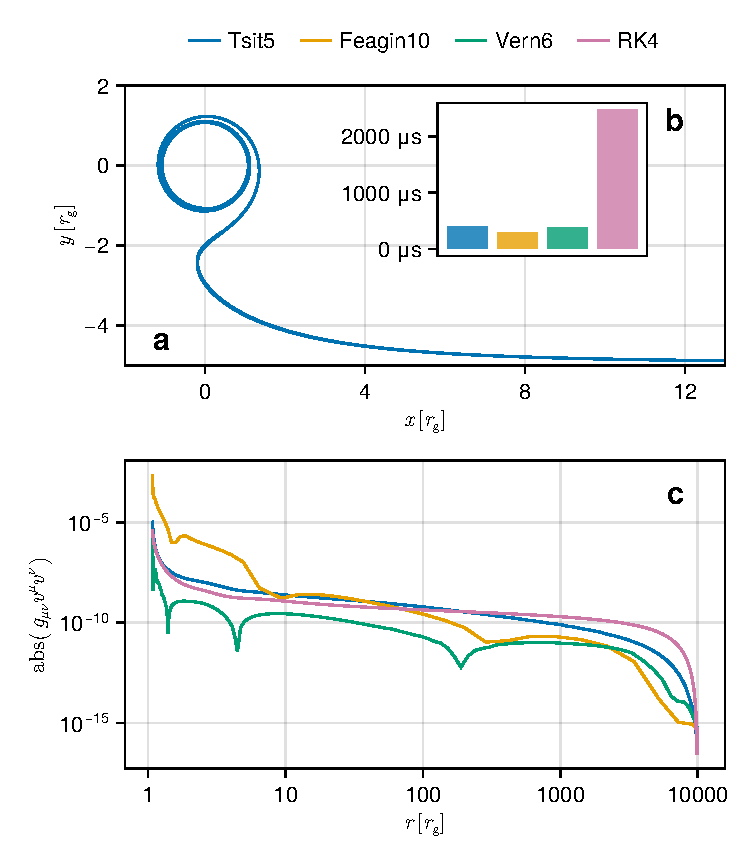
\includegraphics[width=0.95\linewidth]{figures/stability.conservation.pdf}
	\caption{A comparison of different ODE integration algorithms using the default
    tolerances $\text{abstol} = \text{reltol} = 10^{-9}$. Panel a) shows the
    null-geodesic of the Kerr spacetime, $a = 0.998$, for impact parameters
    $\alpha = 5$ and $\beta = 0$ integrated from the starting position $x^r =
    10^4 \rg$ and $x^\theta = \pi / 2$.  . All of the algorithms considered
    yield the same solution. Panel b) shows the integration time for the
    geodesic considered. The integration time is approximately equal for all of
    the algorithms except for RK4. Panel c) shows the value of the conserved
    quantity $g_{\mu \nu} v^\mu v^\nu = 0$ along the trajectory, used as a
    measure of stability of the integration algorithm.
}
	\label{fig:dot-stability}
\end{figure}

To test \emph{accuracy}, we calculate the angular deflection. The deflection is
the difference in $x^\phi$ of a geodesic traveling from positive to negative
infinity, that is
\begin{equation}
	\delta x^\phi :=
		x^\phi_{+\infty} - x^\phi_{-\infty}
		- \pi,
\end{equation}
where $\pi$ is the angular change for a trajectory that experiences no
deflection. Semi-analytic solutions for the deflection angle in the Kerr
spacetime have been calculated for equatorial geodesics in
\cite{iyer_lights_2009}. The authors use elliptical integrals to find the
coordinate differences. We follow their notation and denote the \emph{analytic}
deflection angle $\hat{\alpha}$.

Figure \ref{fig:deflection-angle} shows the deflection angle as a function of
impact parameter $\alpha$, along with a  measure of the error for the different
integration algorithms. There is asymptotic behaviour of the error as $\lvert
\alpha \rvert$ increases. This is related to our approximation of an ``observer
at infinity'' discussed in Section \ref{sec:observers-and-emitters}. As can be
expected, the error increases if $x^r_\text{start}$ is decreased, and
vice-versa. Here we again see the impact that the choice of integrator can have
on numerical errors.

\begin{figure}
	\centering
	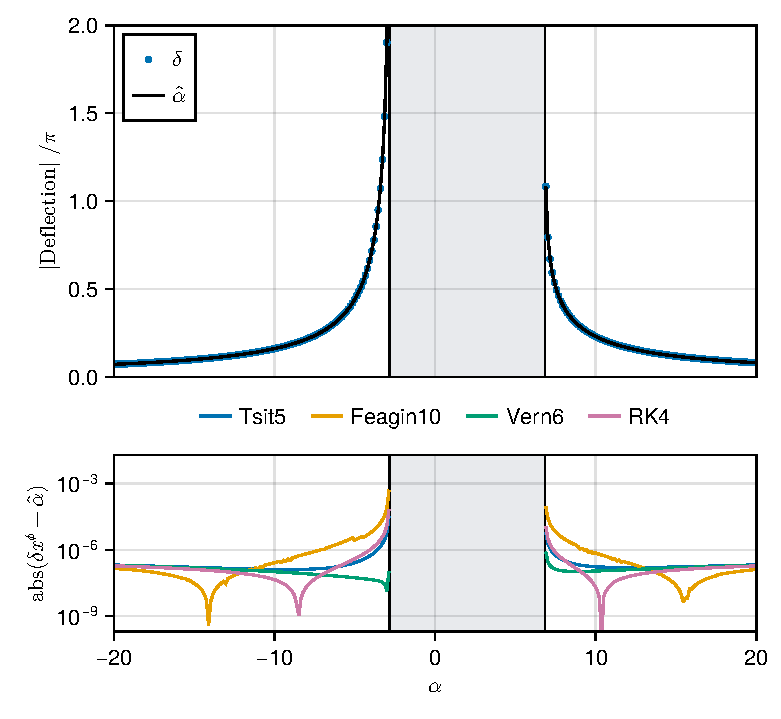
\includegraphics[width=0.94\linewidth]{figures/deflection.iyer-hansen.pdf}
	\caption{Deflection angle in the Kerr spacetime ($M = 1$, $a = 0.998$) for geodesics in the equatorial plane over a range of impact parameters $\alpha$. Upper panel: numerical deflection $\delta x^r$ calculated with  $x^r_\text{start} = 2 \times 10^8 \, \rg$, absolute and relative tolerances set to $10^{-14}$, and effective infinity $4 \times 10^8\, \rg$, shown with the numerical solutions for $\hat{\alpha}$. Lower panel: the absolute relative error between the numeric and analytic deflection angles for different integration algorithms.}
	\label{fig:deflection-angle}
\end{figure}


\todo{Energy conservation, deflection problem, shadow, tests for naked-singularities}


\subsection{Emissivity curves}

To test our implementation of Section \ref{sec:emissivity-profiles}, we
calculate the emissivity profiles on the surface of a thin equatorial accretion
disc illuminated by an on-axis lamppost corona to test our results against
\cite{wilkins_understanding_2012} and \cite{dauser_irradiation_2013}. These are
shown in Figure \ref{fig:emissivity-profiles} and are in good agreement with
published results. Also shown is the effect of the Shapiro delay $t$, on the
arrival time of a photon at a given radius on the disc.

\begin{figure}
	\centering
	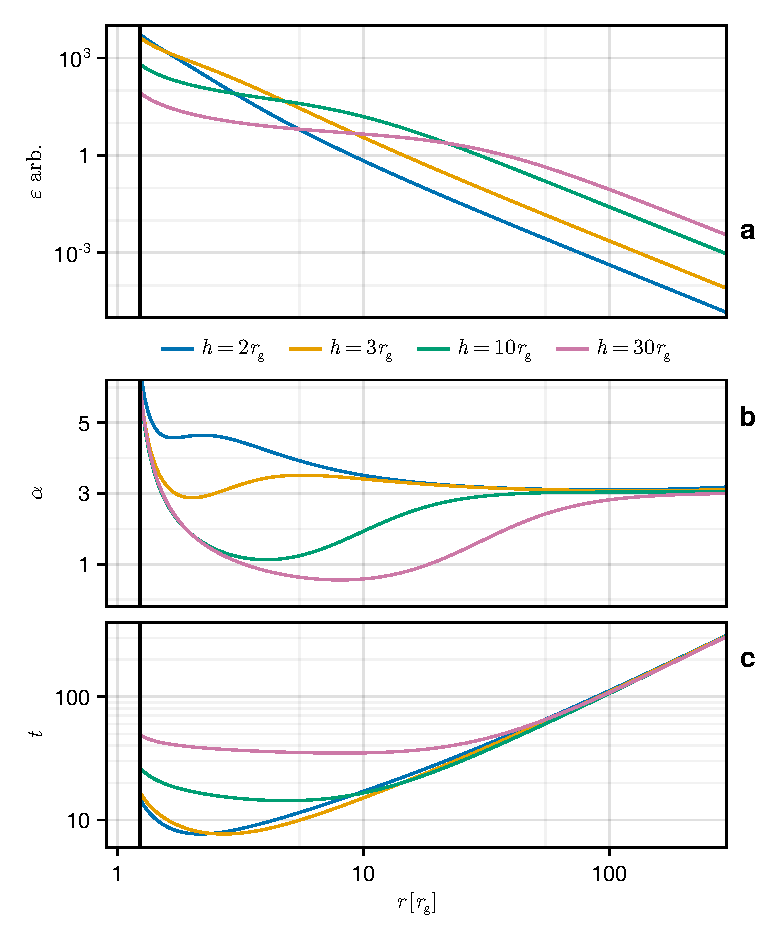
\includegraphics[width=0.99\linewidth]{figures/emissivity.point-source.pdf}
    \caption{Emissivity profiles of a lamppost point source for various heights
        above the spin axis of a maximally spinning Kerr black hole ($a =
        0.998$). Panel a) shows the emissivity profiles in arbitrary flux units.
        Panel b) is the $\alpha$ exponent of the emissivity profile found by
        differentiating the emissivity profile as $r^{-\alpha}$.  Panel a) and
        b) are to be compared to Figures 2 and 3 in
        \citet{dauser_irradiation_2013}. Panel c) is the light-travel time of
        the photon from the lamppost to the disc. The increase in light travel
        time at small radii is due to the strong gravity effects.
}
	\label{fig:emissivity-profiles}
\end{figure}

Modifying the geometry, or adding instantaneous velocities to the corona have
been explored in \cite{gonzalez_probing_2017}. The emissivity curves calculated
are for extended corona are then the time-averaged emissivities on the disc.
These emissivities can be approximately calculated using a Monte-Carlo approach,
by sampling (uniformly) random points in the volume of the corona as the sources
of isotropic emission. The relevant transformations for mapping the local
emission vectors back to the global coordinates is the same as discussed in
Section \ref{sec:observers-and-emitters}.

\subsection{Line profiles}

Transfer functions are integrated as described in Section
\ref{sec:transfer-function-integration}, neglecting the timing components.
Figure \ref{fig:relline-comparison} compares the line profiles computed using
the transfer functions of \Gradus and the \relline model of
\cite{dauser_broad_2010}\footnote{We compare against the \relline v2.3 with
table v0.5a distributed in the Relxill package
\url{http://www.sternwarte.uni-erlangen.de/~dauser/research/relxill/}. These are
the latest versions at time of writing.}. We see good agreement to within $\sim
1\%$ accuracy.

\begin{figure}
	\centering
	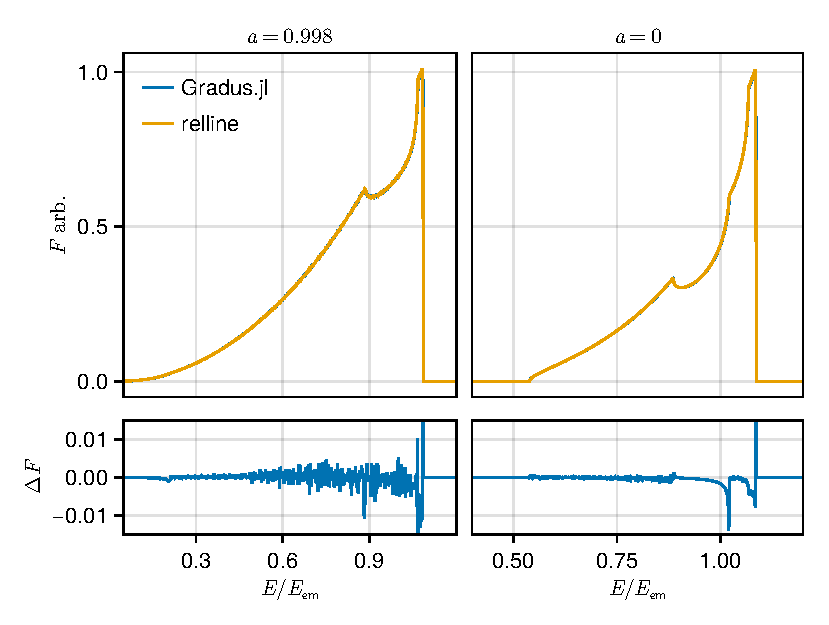
\includegraphics[width=0.99\linewidth]{figures/lineprofiles.comparison.pdf}
	\caption{Comparison of line profiles calculated by integrating transfer functions with emissivity $I_\text{em} = \varepsilon(r_\text{em}) = r_\text{em}^{-3}$ using \Gradus and \relline. The transfer functions are calculated for an observer at $r_\text{obs} = 1000\rg$ and $\theta_\text{obs} = 40^\circ$, and integrated between $r_\text{in} = \risco$ and $r_\text{out} = 50 \rg$. Left panel is the the maximally spinning Kerr spacetime, whereas the right panel is the Schwarzschild spacetime.}
	\label{fig:relline-comparison}
\end{figure}

In addition to comparing to published results, \Gradus offers self-consistent
checks by calculating line profiles using both Cunningham transfer functions and
direct $(\alpha, \beta)$ photon binning. This is useful especially for unusual
disc geometries, where obscuration effects make calculating the Cunningham
transfer functions difficult, as described in
\ref{sec:partially-obscured-functions}. In Figure \ref{fig:line-profile-ssd} we
show line profiles for the \citet{shakura_black_1973} Disc (SSD) model using a fixed power-law emissivity
function, with both numerical methods yielding identical line profiles,
indicating our datum plane method is valid.

\begin{figure}
	\centering
	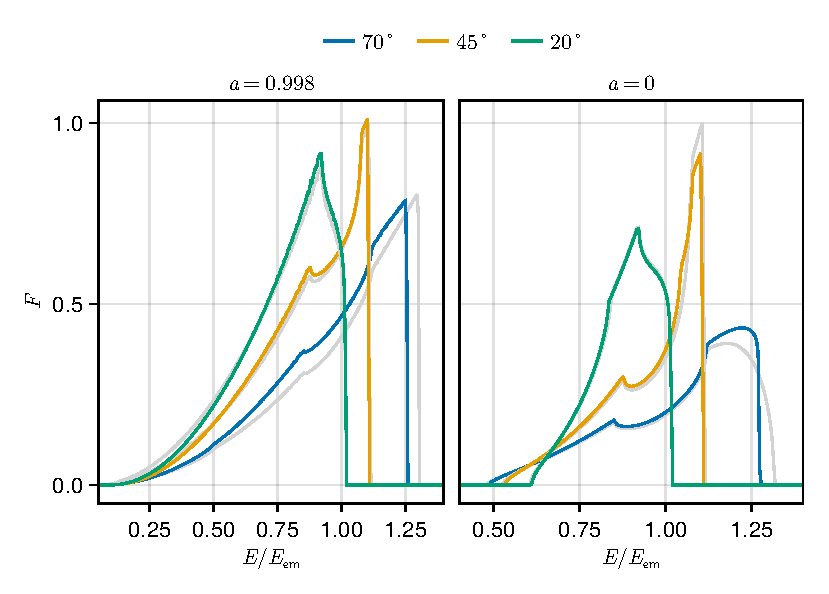
\includegraphics[width=0.99\linewidth]{figures/lineprofiles.ssd.pdf}
	\caption{Line profiles for the SSD with $\dot{M} / \dot{M}_\text{Edd} = 0.3$ for different observer inclinations $\theta_\text{obs}$ and emissivity $I_\text{em} = \varepsilon(r_\text{em}) = r_\text{em}^{-3}$. The transfer functions are calculated as in Figure \ref{fig:relline-comparison}, and integrated over the same limits. The light-grey lines correspond to the geometric thin disc ($\dot{M} / \dot{M}_\text{Edd} = 0$), and differ only for steep inclinations due to obscuration of inner $r_\text{em}$. Left panel is the the maximally spinning Kerr spacetime, whereas the right panel is the Schwarzschild spacetime.}
	\label{fig:line-profile-ssd}
\end{figure}


\subsection{Reverberation lags}
\label{sec:lag-transfer-functions}

AGN and XRBs exhibit a phenomena where the high energy X-ray emission from the
corona is observed both directly and a short delay later after being reprocess
by the accretion disc. The time delay between the direct and reflected
components is increased by the effects of strong gravity on the light travel
time, and therefore depends on properties of the black hole. These lags are
known as \textit{reverberation lags} (see e.g. \cite{uttley_x-ray_2014} or
\cite{cackett_reverberation_2021} for a review). Reverberation lags are
typically expressed as a time lag as a function of Fourier phase frequency of
the driving continuum signal, or as a time lag between energy bands.

Simulating either the lag-frequency or lag-energy spectra involves computing a
set of transfer functions that record the arrival time and observed energy of
each flux element \citep{reynolds_x-ray_1999}. See Figure
\ref{fig:lag-frequency-transfer-functions} for examples. By convention the
origin of the time axis is set to the (mean) arrival time of the continuum
emission. We disambiguate these transfer functions from others by referring to
them as the \textit{lag transfer functions}. They are calculated by re-binning
image planes after ray-tracing the relevant quantities. We devised a method for
calculating the lag transfer functions using the Cunningham transfer functions,
described in \ref{sec:transfer-function-integration}. In this section, we verify
our methods by comparing with results in the literature.

The lag transfer functions depend on the choice of observer inclination,
spacetime, coronal model, and disc model. The inclination of the observer is
sensitive to gravitational lensing effects as well as influencing the relative
distances of different regions of the disc and corona, affecting the arrival
times of emission. The spacetime changes both the light travel time close to the
central singularity and the gravitational redshift. The spacetime is therefore
imprinted in both the energy and arrival time of each flux element.  The coronal
model, in its geometry and spectra, modifies the emissivity profile of the
accretion disc (which in turns changes the flux element coming from each disc
element). The coronal geometry may also change the arrival time of both the
continuum and reflected emissions. The disc geometry contributes to all of the
above.

% \citep{reynolds_x-ray_1999,wilkins_origin_2013,cackett_modelling_2014}

\begin{figure}
	\centering
	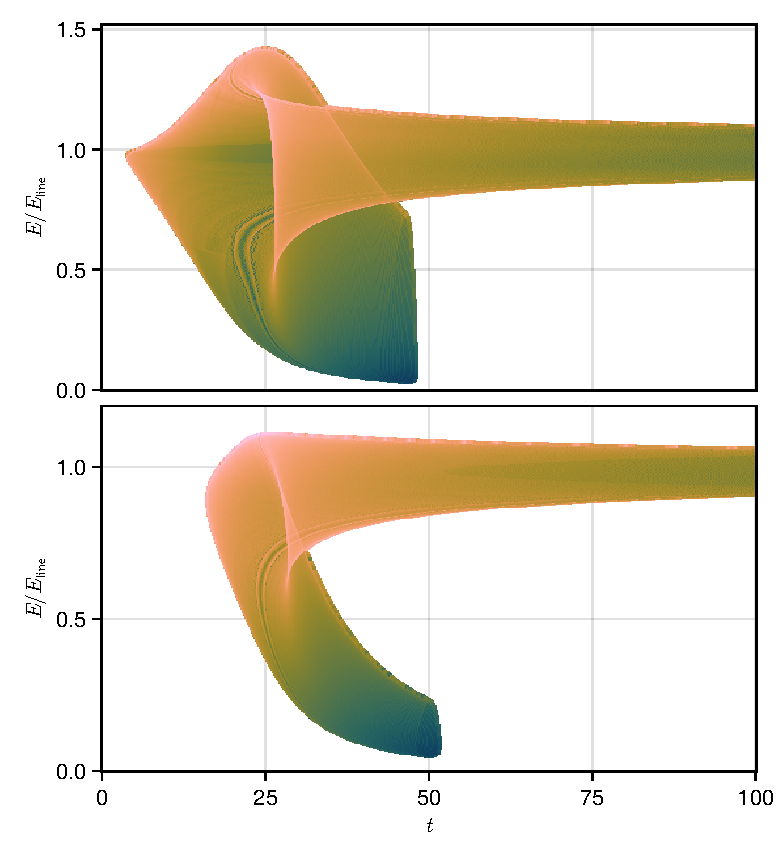
\includegraphics[width=0.97\linewidth]{figures/transfer-functions.2d.pdf}
    \caption{Two-dimensional transfer functions for the maximally spinning Kerr
    spacetime ($a = 0.998$) for two different observer inclinations. These are
    calculated by integrating the time-dependent transfer functions (details in
the text).}
	\label{fig:lag-frequency-transfer-functions}
\end{figure}

\subsubsection{Lag-frequency spectra}

% and allows us to construct high resolution lag transfer functions of
% \cite{reynolds_x-ray_1999} with little additional computational time (see
% Section \ref{sec:lag-transfer-functions}).

Summing the lag transfer functions (Figure
\ref{fig:lag-frequency-transfer-functions}) over the energy axis for a given
energy range yields an \textit{impulse response function} $\psi(t)$, which
encodes how the disc responds to the impulse of a coronal flash. This impulse
response depends on the properties of the illuminating corona, accretion disc,
spacetime, and inclination of the observer. Examples for different lamppost
heights over the full energy range are shown in the top panel of Figure
\ref{fig:reverberation-thin}.

Following \cite{cackett_modelling_2014}, we define the \textit{response
fraction} $R$ as the ratio of reflected to continuum flux. The impulse response
in the Fourier domain is the scaled Fourier transform
\begin{equation}
	\mathscr{F}_\psi(f) := R \int_{0}^\infty \psi(t) \e^{-2\pi i f t} \d t.
\end{equation}
The phase difference between the reflected and continuum flux is
\begin{equation}
	\phi(f) = \tan^{-1} \left(
		\frac{\Im{\mathscr{F}_\psi}}{1 + \Re{\mathscr{F}_\psi}}
	\right),
\end{equation}
where $\Im{\mathscr{F}_\psi}$ and $\Re{\mathscr{F}_\psi}$ are the imaginary and
real components of $\mathscr{F}_\psi$ respectively. The imaginary component
represents the lag contribution to the phase difference. Since the driving
signal is present in both bands, it adds no lag contribution, but serves to
dilute the phase difference and therefore the real component of the signal
through the $+1$ in the denominator. \todo{expand on this}

A subtlety to address here in the normalisation of the impulse responses, as we
do not fully model the continuum spectrum. We assume, as in
\cite{cackett_modelling_2014}, that the reflected flux of the Fe
K$\alpha$ line is equal to the continuum flux ($R = 1$). Therefore, we normalise
the impulse response functions by dividing by a factor $Q = \int \psi_{\text{Fe
K}\alpha}(t)$, so that the area under the \FeKa impulse response function
is unity.


The time lag is defined as
\begin{equation}
	\tau(f) := \frac{\phi}{2 \pi f},
\end{equation}
and relates the observed time lag to the Fourier frequency of the driving signal (lower panel of Figure \ref{fig:reverberation-thin}).

\begin{figure}
	\centering
	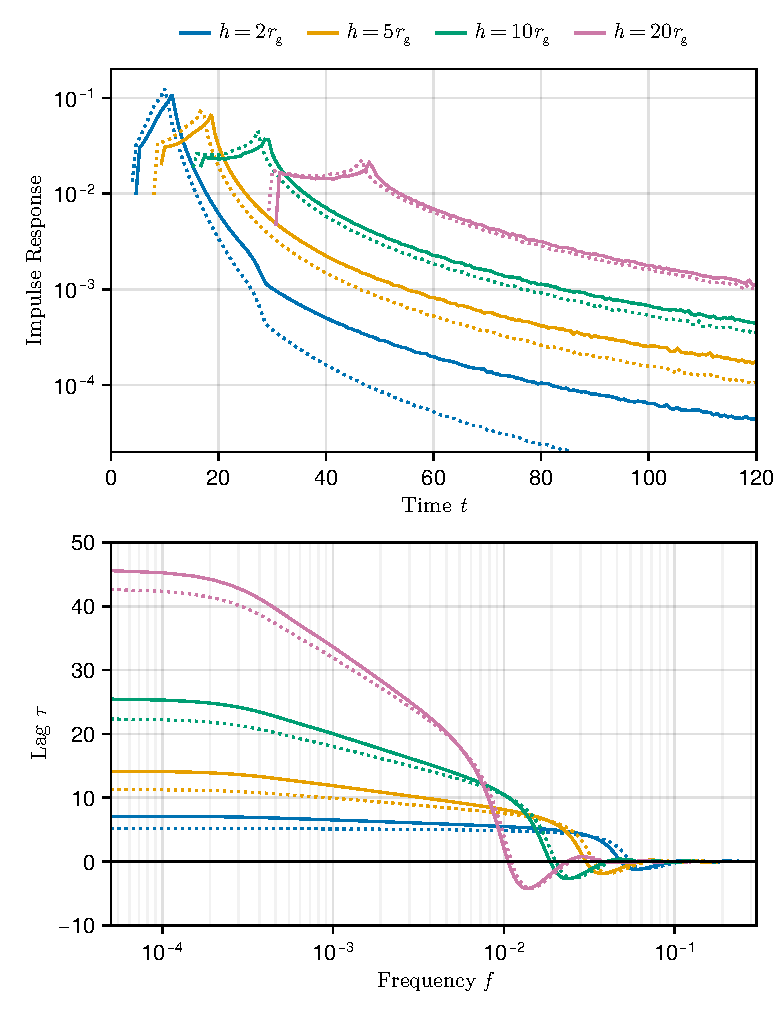
\includegraphics[width=0.98\linewidth]{figures/reverberation.thin-disc.pdf}
    \caption{Impulse responses and lag-frequency spectra of a lamppost model in
        the Kerr spacetime ($a = 0.998$) for different heights of the lamppost
        model. The solid lines are the razor-thin disc case, whereas the dotted
        lines are for the Shakura-Sunyaev disc solution with $\dot{M} /
    \dot{M}_\text{Edd} = 0.3$. Panel a) shows the impulse responses summed
across all energy bands, and panel b) shows the corresponding lag-frequency
spectra of the impulse responses. }
	\label{fig:reverberation-thin}
\end{figure}

We find good agreement with \cite{cackett_modelling_2014} for all cases.

\subsubsection{Lag-energy spectra}

Lag-energy spectra are calculated within specific frequency bands $f + \Delta
f$. Since we have mandated for consistency with \cite{cackett_modelling_2014}
that the reflected flux of the \FeKa line is equal to the continuum flux,
the reference energy band is $E/E_\text{em} = 1$.  For the impulse response of
each energy channel (rows in the lag transfer functions), the lag-frequency
spectrum is calculated. The mean lag within $f + \Delta f$ is determined, and
plotted as a function of energy. In Figure \ref{fig:lag-energy} is illustrated
the time lag as a function of energy relative to the \FeKa band,
to be compared to Figure 11 in \cite{cackett_modelling_2014}. As with the
lag-frequency spectra, we attribute the differences in the low frequency band to
the weak field approximation employed by the other authors, which results in a
larger low frequency lag.

\begin{figure}
	\centering
	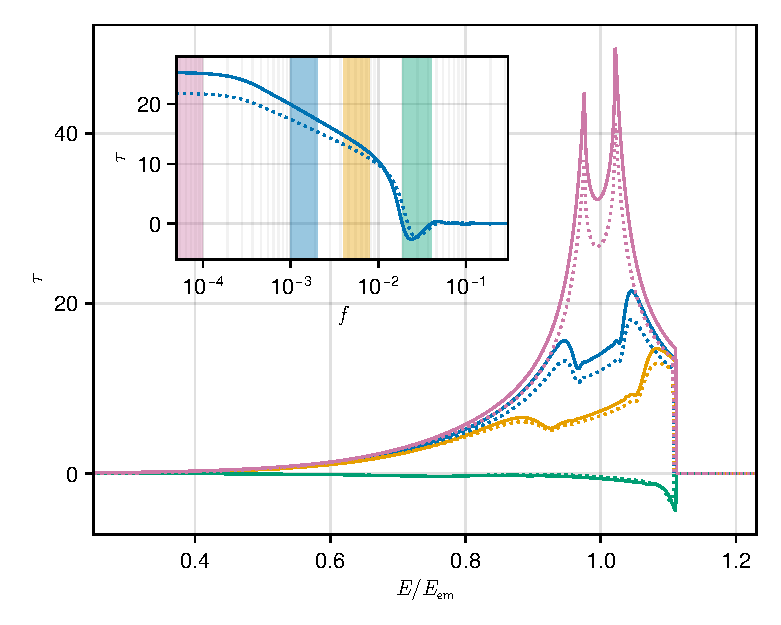
\includegraphics[width=0.98\linewidth]{figures/reverberation.lag-energy.pdf}
	\caption{Lag-energy spectra for the same setup as in Figure
    \ref{fig:reverberation-thin} but only for case where the lamppost height is
$h=10$. The different colours now correspond to the frequency bands used to
calculate the lag-energy spectrum (shown in the inset panel). The solid lines,
as before, denote the razor thin disc, whereas the dotted lines are the
Shakura-Sunyaev disc.}
	\label{fig:lag-energy}
\end{figure}


\subsection{Radiative transfer}

\begin{figure*}
	\centering
	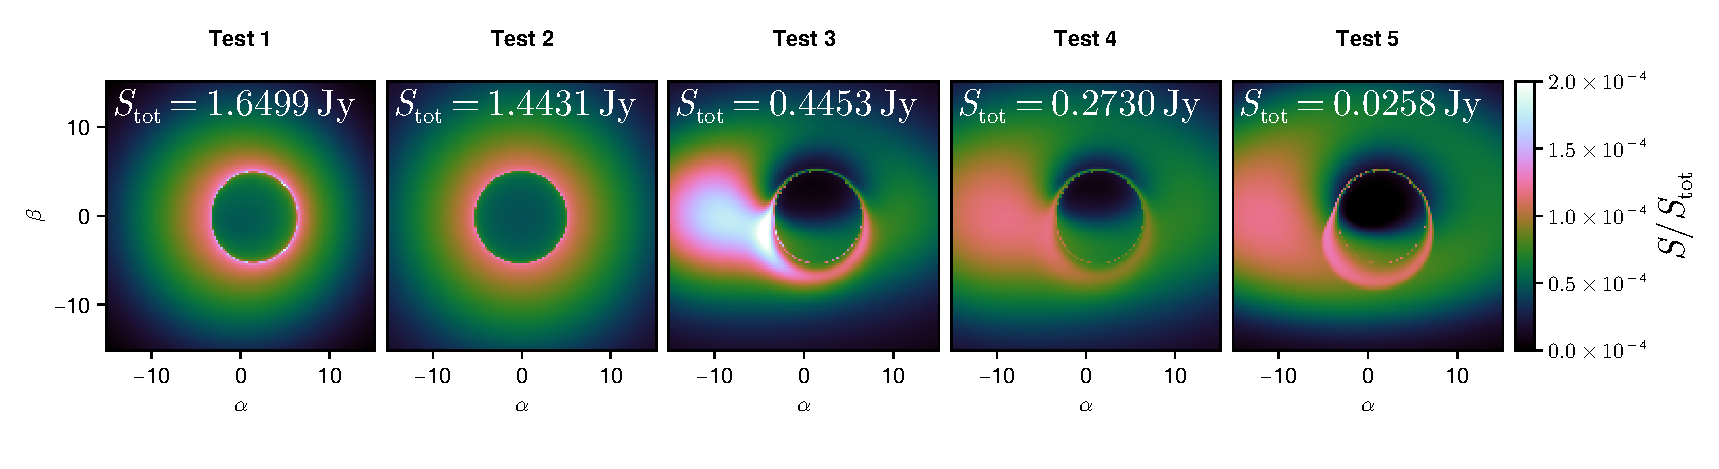
\includegraphics[width=0.99\linewidth]{figures/radiative-transfer.gold.pdf}
	\caption{Intensity images calculated with \Gradus of the radiative transfer analytic test models specified in \citet{gold_verification_2020} with resolution $128 \times 128$ pixels, and impact parameters ranging between $-15\, \rg$ and $15\, \rg$, and observer position $r_\text{obs} = 1000\, \rg$ and inclination $\theta_\text{obs} = 60^\circ$. The test cases correspond to the test parameters in their Table 1. The colouring is the intensity for the geodesic corresponding to that pixel normalized over the total intensity .}
	\label{fig:gold-test-problems}
\end{figure*}

\cite{gold_verification_2020} specify an analytic model for testing radiative
transfer codes (their Section 3.2, with results shown in their Figure 2 and 3).
The model gives the emissivity and absorptivity coefficients of a (corotating)
fluid as a function of radial coordinate. There are five free parameters in this
specification that can be used to control the model, for which they give 5
standardized tests.

We have implemented their model and see very good agreement across all of the
tests, shown in Figure \ref{fig:gold-test-problems}. Our covariant radiative
transfer implementation therefore reproduces the same results as other GRRT
codes to within standard tolerances.

\subsection{Other spacetimes}

\Gradus is designed to allow new spacetime metrics to be implemented easily, and
self-consistently calculates higher-order results within the spacetime.
Reflection and reverberation features have been explored with non-Kerr metrics
by other groups (\todo{cite cosimo's papers}), but approach integrating the
geodesic equation with a mixed-symbolic approach. That is, the Christoffel
symbols are calculated using a computer algebra system (CAS), and the resulting
symbolic expressions are transformed into executable code. This has the
limitation that if the symbolic expressions become too complex for the CAS
system, the methodology breaks down. This can already happen when more than one
deformation parameter is included.

Our approach using AD is robust for metrics that include many deformation
parameters. \Gradus provides the means to build reflection models that can
therefore explore the degeneracies between these parameters, and inform
modelling limitations when studying alternative spacetimes.

To test our methods we compare our results to other published codes for the
Johannsen-Psaltis metric \cite{johannsen_regular_2013}. This metric is not a
strict solution to the Einstein field equations, but is used to quantify
deviations from the Kerr metric using a multipole expansion of \todo{explain}.
The comparison is shown in Figure \ref{fig:compare-johannsen}.

\todo{compare against Johannsen Psaltis paper to show that we get the same line profiles for specific emissivity functions, and compare to Bambi's to show we get the same for self-consistent emissivities}.

\section{Applications}
\label{sec:applications}

The thick disc transfer function calculation method described in Section
\ref{sec:partially-obscured-functions} allows spectra for arbitrary disc
geometries to be efficiently computed. We demonstrate this by calculating high
resolution lag-energy spectra for the SSD, with self consistent emissivity and
light-crossing profiles for the lamppost model. The results are shown in Figure
\ref{fig:reverb-thick-discs} for different Eddington accretion rates. The effect
of the obscuration of the disc is here visible as it is in the lineprofiles; as
the inclination steepens, the blue shifted higher energy component of the
profile moves to lower energy. There is also a decrease in the time lag relative
to the thin disc case which is numerically comparable to the thickness of the
disc. At lower inclinations, the effect of the disc thickness is negligible.
\todo{compare with results of Taylor and Reynolds and Abdikamalov}.

In Figure \ref{fig:reverb-thick-discs-corona}, the lamppost height is changed
for a fixed Eddington ratio. For low coronal heights, the thickness of the disc
has a significant impact on the emissivity and light-crossing profiles, which
therefore distorts the observed lag-energy profile across all inclinations and
Fourier frequencies.

\begin{figure*}
	\centering
	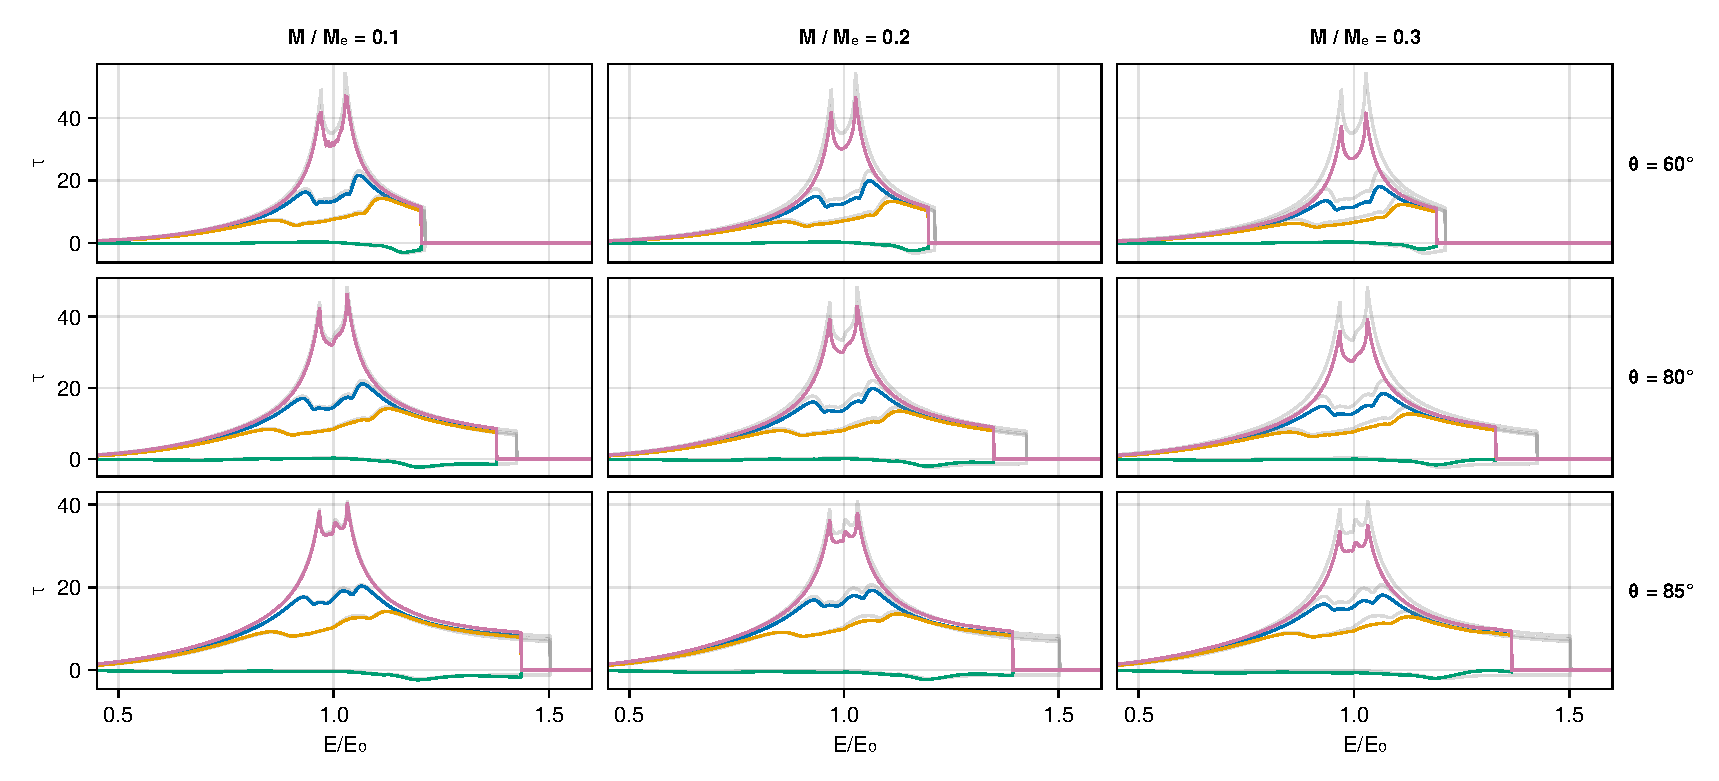
\includegraphics[width=0.99\linewidth]{figures/reverberation.thick-disc.pdf}
    \caption{Lag-energy profiles for the SSD, using the same colour scheme as in
        Figure \ref{fig:lag-energy}. For all figures the Kerr spacetime
        ($a=0.998$) is used with a lamppost corona, $h = 10 \rg$. The light grey
        lines show the corresponding razor-thin disc lag-energy profiles. The
        columns show the effect of changing the Eddington ratio $\dot{M} /
        \dot{M}_\text{Edd}$, and the rows are changing the inclination. When
        $\theta \lesssim 40^\circ$, the differences between the thin disc and
        the SSD are minimal when the lamppost corona is at an appreciable height
        above the black hole.}
	\label{fig:reverb-thick-discs}
\end{figure*}

\begin{figure*}
	\centering
	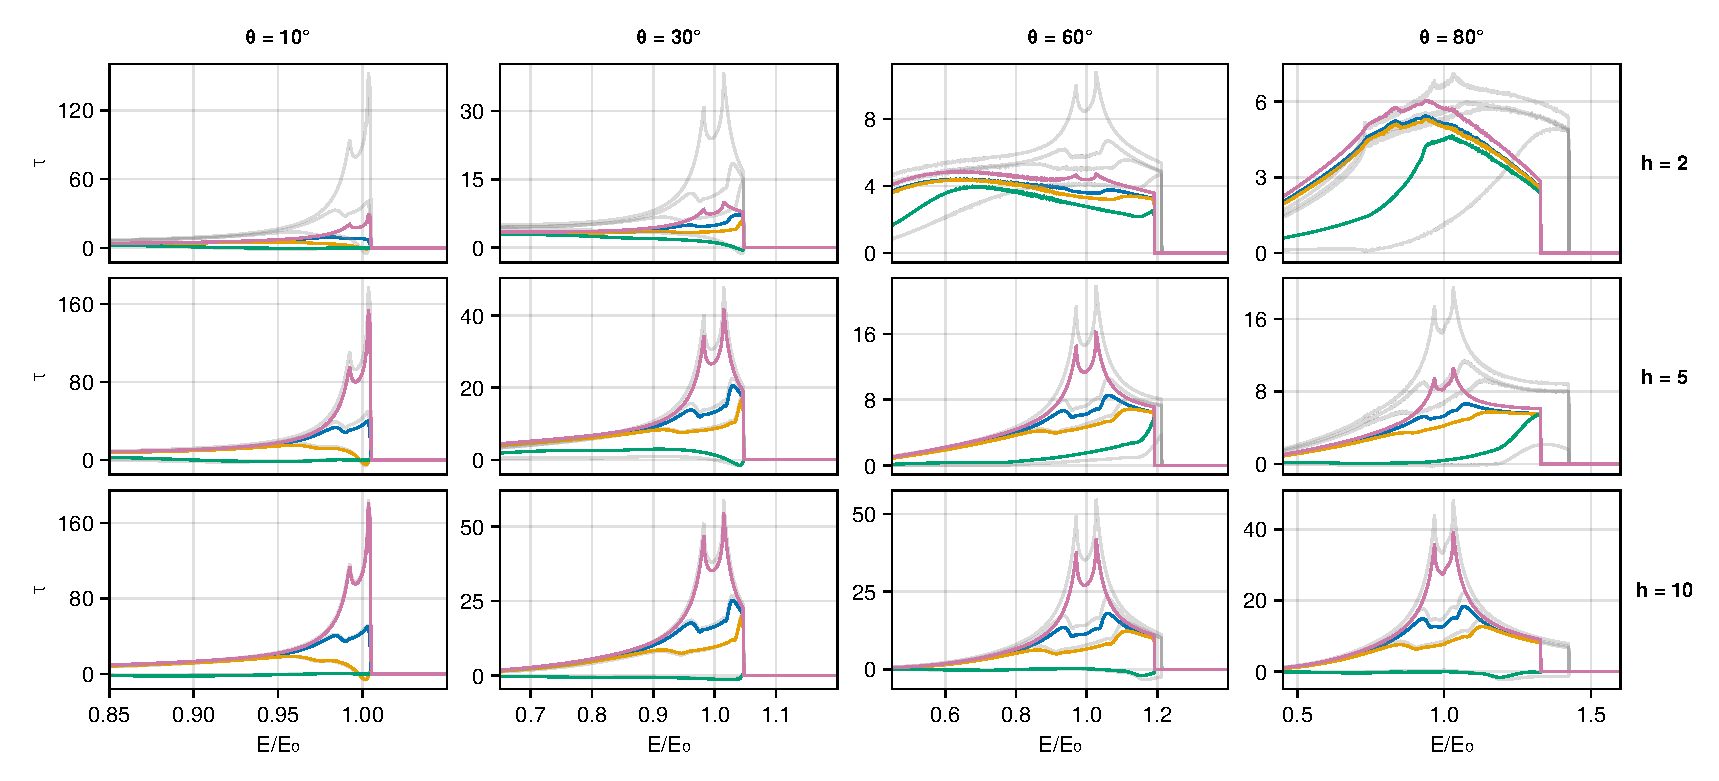
\includegraphics[width=0.99\linewidth]{figures/reverberation.thick-disc-corona.pdf}
    \caption{As in Figure \ref{fig:reverb-thick-discs}, except the Eddington
        ratio is now fixed to $0.3$, and instead the lamppost corona height is
        varied. When the height of the corona is low, there is significant
        obscuration leading to increased emissivity at low radii, and reduced
        emissivity at distant radii, and similarly with the light crossing
    times. This makes a marked change irrespective of inclination, but only
occurs when the coronal height is comparable to the height of the disc.}
	\label{fig:reverb-thick-discs-corona}
\end{figure*}

\Gradus can be used to efficiently generate new reflection and reverberation
models that can be fitted to observational data, and can be tweaked to provide
sufficient resolution for the next generation of high resolution X-ray
spectroscopy observatories, such as XRISM\citneeded. Our software is written to
allow users to be able to generate these models themselves using short scripts,
and compose the different model components together to simulate new systems.

The ability to change the specific black hole solution being simulated has
applications for testing relativity theories, and can expedite the theoretical
modelling process for researchers exploring new gravity theories. The inclusion
of radiative transfer is intended for exploring different emission and
absorption features, and for eventually tracing through the output of general
relativistic magneto hydrodynamic simulations.

We are already in the process of extending our modelling capabilities to
efficiently include additional extended coronal models using a novel
decomposition technique (\todo{Baker \& Young, in prep}), as well as adding
the ability to trace Stokes parameters through a system to calculate
polarization quantities.

\section{Conclusions}
\label{sec:conclusion}

We encourage the community to contact us with interesting problems that may be tackled using \Gradus as we are happy to assist with new applications of the code.

\todo{problems with the code are being patched, see github issues}

\section*{Acknowledgements}
This work is supported by the UKRI AIMLAC CDT funded by grant EP/S023992/1.

We thank Jiachen Jiang, Cosimo Bambi and Askar Abdikamalov for sharing their
software for comparisons, and thank Corbin Taylor for making his
\texttt{fenrir} code, along with many example scripts, public at our request. FB thanks Rosie for her expert debugging assistance. All figures created using Makie.jl \citep{DanischKrumbiegel2021}, using the color scheme of \cite{wong_points_2011}.

%%%%%%%%%%%%%%%%%%%%%%%%%%%%%%%%%%%%%%%%%%%%%%%%%%
\section*{Data Availability}

No new data or analyses have been created for this work. The code to reproduce
this paper and all figures therein is freely available under GPL 3.0 license:
\url{https://github.com/fjebaker/gradus-paper}


% The inclusion of a Data Availability Statement is a requirement for articles published in MNRAS. Data Availability Statements provide a standardised format for readers to understand the availability of data underlying the research results described in the article. The statement may refer to original data generated in the course of the study or to third-party data analysed in the article. The statement should describe and provide means of access, where possible, by linking to the data or providing the required accession numbers for the relevant databases or DOIs.

%%%%%%%%%%%%%%%%%%%% REFERENCES %%%%%%%%%%%%%%%%%%

% The best way to enter references is to use BibTeX:

\bibliographystyle{mnras}
\bibliography{citations} % if your bibtex file is called example.bib


%%%%%%%%%%%%%%%%%%%%%%%%%%%%%%%%%%%%%%%%%%%%%%%%%%

%%%%%%%%%%%%%%%%% APPENDICES %%%%%%%%%%%%%%%%%%%%%

\appendix

\section{orthonormalization with Gram-Schmidt}
\label{appendix:gram-schmidt}

The theorem of Gram-Schmidt states that it is always possible to construct a set of orthonormal vectors in any inner-product space $\mathbb{R}^n$, and uses a projection-subtraction procedure as a proof \citep{schmidt_uber_1989}. Starting with $n$ linearly independent vectors $\vector{v}_n$, and denoting the projection of a vector $\vector{u}$ along the direction of $\vector{v}$ as
\begin{equation}
\mathrm{P}_{\vector{v}}\left(\vector{u}\right) := \frac{\vector{v} \cdot \vector{u}}{\vector{u} \cdot \vector{u}}\ \vector{u} = \frac{g_{\mu\nu} v^\mu u^\nu}{g_{\sigma\rho} u^\sigma u^\rho} \vector{u},
\end{equation}
allows expressing the Gram-Schmidt procedure as
\begin{align}
    \vector{k}_1 &= \vector{v}_1, \nonumber \\
    \vector{k}_2 &= \vector{v}_2 - \mathrm{P}_{\vector{k}_1}\left(\vector{v}_2 \right), \nonumber \\
    &\vdots \nonumber \\
    \vector{k}_n &= \vector{v}_n - \sum_{i = 1}^{n-1} \mathrm{P}_{\vector{k}_i} \left(\vector{v}_n \right).
\end{align}
Constructing meaningful orthonormal frames requires appropriate choice of the initial linearly independent vectors $\vector{v}$, in order to associate global directions with the tetrad. The locally non-rotating frame (LNRF), with angular velocity $\omega = -g_{t\phi} / g_{\phi\phi}$, has tangential frame velocity $v^\mu = A (1, 0, 0, \omega)$ where $A$ is some normalization. To construct the LNRF, a choice of initial vectors may therefore be
\begin{align}
    \vector{v}_1 &= \left(1, 0, 0, \omega \right) \mapsto \dtensor{\e}{(t)}{\mu}, \nonumber \\
    \vector{v}_2 &= \left(1, 0, 0, 1\right) \mapsto \dtensor{\e}{(\phi)}{\mu}, \nonumber \\
    \vector{v}_3 &= \left(1, 1, 0, 1\right) \mapsto \dtensor{\e}{(r)}{\mu}, \nonumber \\
    \vector{v}_4 &= \left(1, 1, 1, 1\right) \mapsto \dtensor{\e}{(\theta)}{\mu},
\end{align}
where we have denoted the corresponding tetrad vector generated by the orthonormalization procedure after the arrow.

Other sensible frames require different initial vectors, and care must be taken in implementing a method that correctly reorders the resulting tetrad vectors: for example, the zero angular momentum (ZAMO) frame for an on-axis coronal source with velocity $\dot{x}^\mu = (1, \d r / \d t, 0, 0)$ requires
\begin{align}
    \vector{v}_1 &= \left(1, \d r / \d t, 0, 0 \right) \mapsto \dtensor{\e}{(t)}{\mu}, \nonumber \\
    \vector{v}_2 &= \left(1, 1, 0, 0\right) \mapsto \dtensor{\e}{(r)}{\mu}, \nonumber \\
    \vector{v}_3 &= \left(1, 1, 1, 0\right) \mapsto \dtensor{\e}{(\theta)}{\mu}, \nonumber \\
    \vector{v}_4 &= \left(1, 1, 1, 1\right) \mapsto \dtensor{\e}{(\phi)}{\mu}.
\end{align}

Our implementation of the Gram-Schmidt procedure is accurate up to machine-level with the analytic tetrads for the LNRF in \cite{bardeen_rotating_1972}, their Equation (3.2), and for the moving source ZAMO frame in \cite{gonzalez_probing_2017}, their Equation (10).

\section{Keplerian orbits of static, axis-symmetric spacetimes with accelerated geodesics}
\label{appendix:circular-orbits}
% \section{Semi-analytic deflection angle for static, axis-symmetric spacetimes}
\label{appendix:deflection-angle}


\section{On the numerical errors in the choice of ODE integrator}
\label{appendix:solvers}

Efforts to compare GRRT codes inevitably face the same problem; that analytic (`true') results to compare to can only be constructed for contrived or simplified models. Instead, there is a tendency to attempt to compare geodesic calculations, often nearing machine precision, as a method of evaluating the accuracy of a given code. A particular fallacy is that calculating with arbitrary precision floating point numbers will in some sense convey a result that is closer to the `truth'. There is however inherent bias in this approach, as the choice of integrator for precisely the same configuration contributes an error that can be significant.

A recent paper showed the choice of ingoing and out-going Eddington-Finkelstein coordinates contributes certain errors in certain GRRT problems, in particular for geodesics close to the event horizon. The magnitude of these errors, however, is far smaller than the difference in choice of integrator.

Taking a different number of steps close to the event horizon alters the floating point error due to the non-commutativity of floting point operations.

\todo{\cite{Rackaukas} has investigated Runge-Kutta tableaus }

\todo{We conclude codes that agree to within $\sqrt{\varepsilon}$...}


% \section{Caution against a weak field approximation}
\label{appendix:continuum-time}

A weak field approximation for general relativistic effects is sometimes used in the interest of computational performance. For example, a spherical radius $R$ outside of which relativistic effects are said to be negligible, such that a flat (Minkowski) spacetime metric is used for ray-tracing and other calculations. In \citet{cackett_modelling_2014}, $R = 100\, \rg$ is used when calculating lag-frequency and lag-energy spectra. However, this approximation introduces a slight error when calculating the light travel time of flux from the disc and continuum source, which has a surprisingly significant effect on the computed lag-frequency spectra.

Since \Gradus is metric agnostic, we implement a new spacetime that switches to the Minkwoski form beyond $R$ and recalculate the lag-frequency relations. Our implementation preserves constant of motions across the boundary when switching from one metric to another, though other weak-field approximations may not, introducing additional errors in the trajectories of geodesics that depend on the ODE integration algorithm used and the solver steps over the boundary.

% The use of this weak-field approximation reproduces the results of \citet{cackett_modelling_2014}, but differs from the lag-frequency curve presented in this paper. We offer the following explanation:

% In cases where the source height above the black hole is small, the systematic error from the weak field approximation between the reflected and continuum flux is approximately equal, and therefore is negligible when the difference in arrival time is calculated, as in
% \begin{equation}
%     \Delta t = \tilde{t}_\text{reflected} - \tilde{t}_\text{continuum} ,
% \end{equation}
% where the tilde denotes the inclusion of some $\delta t$ due to the weak field approximation $\tilde{t} = t_\text{true} - \delta t$. However, when the source height is of appreciable value, say $h > 10\rg$, then for an off axis observer the systematic error introduced by $\delta t$ is greater for the continuum emission than for the reflected component (see Figure \ref{fig:app:weak-field-approx}), resulting in the continuum flux arriving seemingly too early. Note that $\delta t$ is dependant on the observer's position, and decreases with increasing $r_\text{obs}$.

% Figure \ref{fig:app:continuum-time} illustrates the relationship between coronal source height and $\delta t$, calculated by using the weak field approximation at different $R$ and subtracting the equivalent `true' light travel time $t$ (equivalent to $R \rightarrow \infty$). Even at $h = 100$, the continuum flux from the corona is seen to arrive significantly early.

% \begin{figure}
% 	\centering
% 	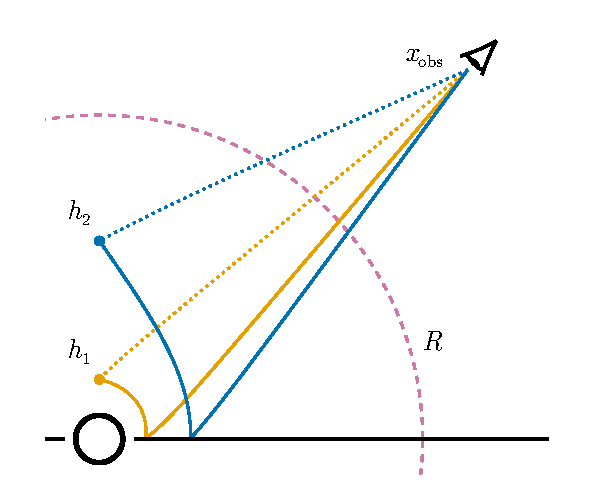
\includegraphics[width=0.80\linewidth]{figures/continuum-time.figure.pdf}
% 	\caption{\todo{TODO}}
% 	\label{fig:app:weak-field-approx}
% \end{figure}

% For the source heights of $h=10\, \rg$ and $h = 20 \rg$ and an observer inclination of $\theta_\text{obs} = 45^\circ$, the path length of the traject

% \todo{a heatmap showing $\delta t$ for different $h$ and observer distances?}

% \begin{figure}
% 	\centering
% 	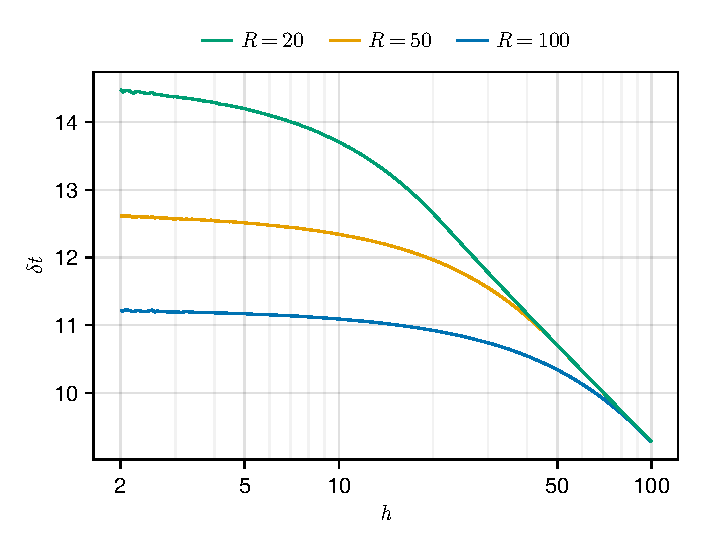
\includegraphics[width=0.98\linewidth]{figures/continuum-time.weak-field.pdf}
% 	\caption{\todo{TODO}}
% 	\label{fig:app:continuum-time}
% \end{figure}

% \section{Hello World}
\label{appendix:hamiltonian-formalism}


% \section{Some extra material}

%%%%%%%%%%%%%%%%%%%%%%%%%%%%%%%%%%%%%%%%%%%%%%%%%%


% Don't change these lines
\bsp	% typesetting comment
\label{lastpage}
\end{document}

% End of mnras_template.tex
